% MidlineSparse: probabilistic foundations (priors, validity, two-stage status)
% Upload this single file to Overleaf. Compile with pdfLaTeX (TeX Live 2022+).
\documentclass[11pt,a4paper]{article}

\usepackage[margin=1in]{geometry}
\usepackage{amsmath,amssymb,amsthm,bm,mathtools}
\usepackage{booktabs,enumitem,microtype,xcolor,hyperref}
\usepackage{tikz}
\usetikzlibrary{arrows.meta,positioning,fit,calc}

\hypersetup{colorlinks=true,linkcolor=blue!50!black,citecolor=blue!50!black,urlcolor=blue!60!black}

\theoremstyle{plain}
\newtheorem{theorem}{Theorem}[section]
\newtheorem{proposition}[theorem]{Proposition}
\newtheorem{lemma}[theorem]{Lemma}
\newtheorem{corollary}[theorem]{Corollary}
\theoremstyle{definition}
\newtheorem{definition}[theorem]{Definition}
\newtheorem{assumption}[theorem]{Assumption}
\newtheorem{remark}[theorem]{Remark}
\theoremstyle{remark}
\newtheorem{caution}[theorem]{Caution}

\newcommand{\R}{\mathbb{R}}
\newcommand{\E}{\mathbb{E}}
\newcommand{\Var}{\mathrm{Var}}
\newcommand{\Ncal}{\mathcal{N}}
\newcommand{\GP}{\mathcal{GP}}
\newcommand{\D}{\mathcal{D}}
\newcommand{\tht}{\theta}
\newcommand{\Th}{\Theta}
\newcommand{\sigmoid}{\operatorname{sigmoid}}
\newcommand{\softplus}{\operatorname{softplus}}
\newcommand{\Kmax}{K_{\max}}
\newcommand{\ind}{\mathbf{1}}
\newcommand{\law}{\mathrm{Law}}
\newcommand{\EBMAP}{EB--MAP}
\newcommand{\simplex}{\Delta}

\title{\textbf{What Prior Does MidlineSparse Impose?}\\[0.35em]
\large Probabilistic Status of Two-Stage Non-Gaussian GP UQ\\[0.25em]
\normalsize Matching \texttt{gpplus/models/midline\_sparse\_moe.py}}
\author{SpectralGPPlus / experiments\_MOEGP\\
Critical note for Overleaf}
\date{\today}

\begin{document}
\maketitle

\begin{abstract}
MidlineSparse is a \emph{two-stage} procedure: (i)~fit and freeze an exact Gaussian-process (GP)
midline; (ii)~fit a sparse Gaussian mixture of residual experts on top.
This note answers, with proofs and explicit caveats: \textbf{What prior is imposed on the
solution?} and \textbf{Is what the model recovers a valid probabilistic object?}
The full Bayesian card (priors, likelihood, posterior, conditionals) is
Section~\ref{sec:bayes-spec}.
The fitted object is an
\emph{empirical-Bayes maximum a posteriori} (\EBMAP) estimative predictive
(Definitions~\ref{def:ebmap}--\ref{def:estimative}) when usage/alive/merge are off;
with those controllers on, it is a \emph{controller-modified} estimative MoG predictive
(Theorem~\ref{thm:honest}).
It is not a Bayesian posterior predictive.
The short answers are:
\begin{enumerate}[leftmargin=1.4em,itemsep=0.2em]
  \item Stage~1 imposes a standard GP prior on a latent function \(f_0\) and yields a
        Gaussian posterior predictive that is used as an \emph{estimative} midline
        \((\mu_0,\sigma_0)\).
  \item Stage~2 does \emph{not} define a Bayesian posterior over functions. It defines a
        parametric family of conditional densities \(p_\tht(y\mid x)\) (mixtures of
        Gaussians---not mixtures of GPs; Section~\ref{sec:mog-vs-mogp})
        trained by \emph{penalized maximum likelihood} (Hard-Concrete \(L_0\)-style
        complexity), optionally plus non-Bayesian controllers (usage, alive, adaptive merge).
        Mixture weights are \(\pi_k(x)\), not \(\pi_k(x)\alpha_k\).
  \item For any fixed parameter \(\tht\) with \(\pi(x)\in\simplex^{\Kmax-1}\) and
        \(v_k(x)>0\), the Stage~2 object \(p_\tht(y\mid x)\) \emph{is} a valid
        conditional probability density. Moments from the law of total variance are then
        well-defined. What is \emph{not} generally valid is interpreting the fitted object
        as \(p(y\mid x,\D)\) under a single coherent hierarchical Bayesian model.
\end{enumerate}
\end{abstract}

\tableofcontents
\newpage

%==============================================================================
\section{Notation conventions}
\label{sec:notation}
%==============================================================================

\begin{center}
\renewcommand{\arraystretch}{1.12}
\begin{tabular}{@{}lp{10.6cm}@{}}
\toprule
Symbol & Meaning \\
\midrule
\(\D=\{(x_i,y_i)\}_{i=1}^n\), \(X\), \(Y\) &
  Training data; inputs; responses \\
\(\simplex^{K-1}\) &
  Probability simplex \(\{w\in[0,1]^K:\sum_k w_k=1\}\) \\
\(f_0\sim\GP(m_0,k_\phi)\) &
  Latent midline GP; mean function \(m_0\), kernel hypers \(\phi\) \\
\((\mu_0,\sigma_0)\) &
  Stage~1 GP posterior predictive mean / std (frozen in Stage~2) \\
\(\sigma_{\mathrm{env}}\) &
  Envelope std in the \emph{hierarchical} MoG; prior-level hyperfield.
  Algorithmic plug-in: \(\sigma_{\mathrm{env}}\leftarrow\sigma_0\) \\
\(\tht=(a,g,\psi_\pi,\psi_\delta)\) &
  Stage~2 parameters (HC logits, carve logits, gate MLP, offset MLP) \\
\(\alpha_k(a)\in[0,1]\), \(\gamma_k=\sigmoid(g_k)\) &
  Expert switch; variance carve-out \\
\(\pi(x)\in\simplex^{\Kmax-1}\), \(\tilde\delta_k(x)\) &
  Gate weights; \emph{pinned} residual offsets \\
\(\mu_k,v_k\) (alias \(\mathrm{Var}_k\)) &
  Expert mean / variance; \(v_k=\sigma_{\mathrm{env}}^2(1-\alpha_k\gamma_k)+\varepsilon\) \\
\(\beta_k\) vs \(\beta_{\mathrm{HC}}\) &
  Optional free expert scale (\(\beta_k\equiv 1\) in champion) vs Hard-Concrete stretch \\
\(m_{\mathrm{merge}}\in[0,1]\) &
  Adaptive merge pressure (controller; not a prior).
  Written \(m\) only when unambiguous \\
\(\Pi=\Phi_\# p(f_0,\tht)\) &
  Pushforward prior on MoG conditionals (Section~\ref{sec:derive-prior}) \\
\EBMAP &
  Empirical Bayes + maximum a posteriori (Definition~\ref{def:ebmap}) \\
\bottomrule
\end{tabular}
\end{center}

\begin{caution}[Canonical generative vs.\ algorithmic specialization]
In the coherent hierarchy, component fields use \((f_0,\sigma_{\mathrm{env}})\).
The implemented two-stage code specializes
\(f_0\leftarrow\mu_0\) and \(\sigma_{\mathrm{env}}\leftarrow\sigma_0(\D)\)
(Definition~\ref{def:estimative}). Identifying \(\sigma_{\mathrm{env}}\) with
\(\sigma_0(\D)\) is an \emph{estimative} step, not a claim that Stage~1 posterior
variance is part of the \(\D\)-free prior \(\Pi\).
\end{caution}

%==============================================================================
\section{Advisor-facing answer: is ``the prior'' a GP?}
\label{sec:advisor}
%==============================================================================

\begin{center}
\fbox{\parbox{0.92\textwidth}{\centering\large\bfseries
No.\quad The prior for MidlineSparse \emph{as a whole} is not ``a GP.''\\[0.35em]
\normalsize\normalfont
A GP prior is used only for the Stage~1 midline latent \(f_0\).
The object returned for non-Gaussian UQ is an \emph{\EBMAP\ / controller-modified
estimative MoG density} on that frozen midline
(Definitions~\ref{def:ebmap}--\ref{def:estimative}, Theorem~\ref{thm:honest}).
}}
\end{center}

\vspace{0.75em}

An advisor asking for mathematical rigor typically wants a clear answer to:
\begin{quote}
\emph{Before seeing data, what random object is the model a prior over?
After seeing data, what posterior (or other) object is recovered?}
\end{quote}
Those questions have \textbf{different answers} for Stage~1 alone versus the full
two-stage MidlineSparse procedure. Conflating them (``the prior is a GP'') is
incorrect for the multimodal UQ claim.

\subsection{Three rigorously distinct objects}
\begin{definition}[Object A --- Stage-1 Bayesian GP]
Prior: \(f_0\sim\GP(m_0,k_\phi)\).\\
Likelihood: \(Y\mid f_0,X\sim\Ncal(f_0(X),\sigma_\varepsilon^2 I)\).\\
Recovered (given type-II ML hypers): Gaussian posterior predictive
\(p(y\mid x,\D,\hat\phi,\hat\sigma_\varepsilon)=\Ncal(\mu_0(x),\sigma_0^2(x))\).
\end{definition}

\begin{definition}[Object B --- Stage-2 parametric family]
For frozen \((\mu_0,\sigma_0)\), a deterministic map
\(\tht\mapsto p_\tht(y\mid x)\) given by the Gaussian mixture
\eqref{eq:mix}. No measure \(p(\tht)\) is sampled; \(\hat\tht\) minimizes NLL\(+R\).
\end{definition}

\begin{definition}[Object C --- Reported MidlineSparse predictive]
\[
  \hat p(y\mid x)
  :=
  p_{\hat\tht}\!\bigl(y\mid x;\,\mu_0,\sigma_0\bigr).
\]
This is a \textbf{probability density in \(y\)} (Theorem~\ref{thm:valid-density}),
but it is \textbf{not} Object~A's posterior predictive, and it is \textbf{not}
obtained by Bayes' rule under a single prior on ``the solution.''
\end{definition}

\begin{theorem}[Why ``the prior is a GP'' fails for MidlineSparse UQ]
\label{thm:not-just-gp}
Suppose the scientific claim is that MidlineSparse provides a non-Gaussian
conditional predictive \(\hat p(y\mid x)\). Then:
\begin{enumerate}[label=(\roman*)]
  \item The GP prior \eqref{eq:gp-prior} alone induces only Gaussian predictives
        of the form \eqref{eq:stage1-pred}. It cannot be ``the prior'' for a
        multimodal mixture predictive.
  \item Object~C is not equal to Object~A's posterior predictive unless
        \(\Kmax=1\) or all residual experts are inactive (\(\alpha_k\tilde\delta_k\equiv 0\)
        and \(\gamma_k\equiv 0\) in the relevant sense).
  \item Therefore any rigorous write-up must state either
        \begin{itemize}
          \item \textbf{(Algorithmic:)} MidlineSparse is a two-stage estimator of
                \(p^\star(y\mid x)\), with Stage~1 a GP and Stage~2 a penalized
                mixture --- \emph{not} a fully Bayesian model; or
          \item \textbf{(Hierarchical Bayesian completion:)} an explicit joint prior
                \(p(f_0,\tht)\) as in Section~\ref{sec:derive-prior}, of which the
                code is only a plug-in approximation.
        \end{itemize}
\end{enumerate}
\end{theorem}

\begin{proof}
(i)~Under \eqref{eq:gp-prior}--\eqref{eq:obs}, the observation-scale predictive at a
test point is Gaussian \citep{RasmussenWilliams2006}. A Gaussian density on \(\R\)
has at most one mode; it cannot represent a general multimodal \(p^\star(y\mid x)\).

(ii)~By Definition of Object~C and \eqref{eq:mix}, if some \(\alpha_k\tilde\delta_k\not\equiv 0\)
with positive \(\pi_k\), then \(p_{\hat\tht}(\cdot\mid x)\) is a nontrivial mixture and
differs from \(\Ncal(\mu_0,\sigma_0^2)\) as measures (e.g.\ they disagree on number of
modes or on kurtosis).

(iii)~Follows: either abandon the claim that a single Bayesian prior generates
Object~C, or supply the missing hierarchical prior and admit the algorithm is an
approximation to that model's posterior predictive.
\end{proof}

\subsection{What to tell an advisor in one paragraph}
\begin{quote}
\emph{Stage~1 places a Gaussian-process prior on a latent midline function and
returns a Gaussian estimative predictive \((\mu_0,\sigma_0)\). Stage~2 does not update
that GP posterior. It fits a sparse Gaussian-mixture residual model by penalized
maximum likelihood (Hard-Concrete \(L_0\) surrogate, offset ridge), optionally plus
non-Bayesian capacity/merge controllers. The quantity we report for UQ is the
estimative MoG \(p_{\mu_0,\hat\tht}(y\mid x)\) (Object~C): valid as a density, but not
the posterior predictive of a single GP nor (under champion controllers) pure
\EBMAP. If a fully Bayesian story is required, the prior must be stated jointly
over \((f_0,\tht)\) and the posterior predictive integrated
(Section~\ref{sec:code-to-posterior}).}
\end{quote}

\subsection{Pointer}
The Bayesian specification (priors, likelihood, posterior, conditionals) is
Section~\ref{sec:bayes-spec}.
The constructive derivation of those priors from the Stage~2 penalties is
Section~\ref{sec:derive-prior}.

%==============================================================================
\section{Bayesian specification: priors, likelihood, posterior, conditionals}
\label{sec:bayes-spec}
%==============================================================================

This section states the MidlineSparse model in standard Bayesian hierarchical form.
Two layers must be kept separate:
\begin{enumerate}[leftmargin=1.4em,itemsep=0.15em]
  \item the \textbf{coherent hierarchical model} one can write on
        \((f_0,\tht,Z,Y)\);
  \item the \textbf{two-stage algorithm}, which is an empirical-Bayes / MAP
        \emph{approximation} to that model (and adds non-Bayesian controllers).
\end{enumerate}
Usage, alive, and adaptive merge are \textbf{not} part of the Bayesian model below
(Section~\ref{sec:merge}); they modify the estimator only.

\subsection{Data, latents, and parameters}
\begin{definition}[Observables and unknowns]
\begin{align*}
  \D &= \{(x_i,y_i)\}_{i=1}^n,
  &
  X &= (x_1,\ldots,x_n),
  &
  Y &= (y_1,\ldots,y_n)^\top,
  \\
  f_0
  &:
  \R^d\to\R
  &&
  \text{(latent midline function)},
  \\
  \tht
  &=
  (a,g,\psi_\pi,\psi_\delta)
  &&
  \text{(Stage-2 parameters; Def.\ below)},
  \\
  Z
  &=
  (z_1,\ldots,z_n),
  \quad
  z_i\in\{1,\ldots,\Kmax\}
  &&
  \text{(latent expert assignments)}.
\end{align*}
Optional hyperparameters: kernel/noise \((\phi,\sigma_\varepsilon)\) for the GP midline,
and ridge / Hard-Concrete scales \((\lambda_\alpha,\lambda_\delta,\ldots)\).
Champion treats \((\phi,\sigma_\varepsilon)\) by type-II ML (empirical Bayes) and treats
\((\lambda_\alpha,\lambda_\delta)\) as fixed.
\end{definition}

\begin{definition}[Deterministic maps from \(\tht\)]
Hard-Concrete / sigmoid maps and networks induce
\begin{align*}
  \alpha_k
  &=
  \alpha_k(a_k)
  \in[0,1],
  &
  \gamma_k
  &=
  \sigmoid(g_k)
  \in(0,1),
  \\
  \pi(x)
  &=
  \mathrm{softmax}\bigl(g_{\psi_\pi}(x)\bigr)
  \in\simplex^{\Kmax-1},
  &
  \delta_k(x)
  &=
  \bigl[\delta_{\psi_\delta}(x)\bigr]_k,
\end{align*}
with \(\tilde\delta(x)\) the pinned version of \(\delta(x)\) so that
\(\sum_k\pi_k(x)\alpha_k\tilde\delta_k(x)=0\) (Section~\ref{sec:pin}).
Component fields (champion \(\beta\equiv 1\)):
\begin{equation}
  \begin{aligned}
  \mu_k(x)
  &=
  f_0(x)+\alpha_k\,\tilde\delta_k(x),
  \\
  v_k(x)
  &=
  \sigma_{\mathrm{env}}^2(x)\,(1-\alpha_k\gamma_k)+\varepsilon,
  \qquad
  \varepsilon=10^{-6}.
  \end{aligned}
  \label{eq:bayes-comp}
\end{equation}
Here \(\sigma_{\mathrm{env}}^2(x)\) is an \emph{envelope variance} field.
In the implemented two-stage code it is the frozen Stage~1 predictive variance
\(\sigma_0^2(x)\). In a fully joint hierarchy one may instead take a constant noise
floor, a parametric envelope, or \(\sigma_{\mathrm{env}}^2\equiv\sigma_\varepsilon^2\);
the Bayesian factorization below does not require identifying the envelope with a GP
posterior variance, only that \(v_k(x)>0\).
\end{definition}

\subsection{Prior}
\begin{definition}[Joint prior on unknowns]
\label{def:bayes-prior}
Under fixed hyperparameters,
\begin{equation}
  \boxed{
  p(f_0,\tht)
  =
  p(f_0\mid\phi)\,p(\tht)
  =
  \GP(f_0;\,m_0,\,k_\phi)
  \;
  p(a)\,p(g)\,p(\psi_\pi)\,p(\psi_\delta)
  }
  \label{eq:bayes-prior}
\end{equation}
with product factors identified from Stage~2 regularizers that do not depend on \(Y\)
through usage statistics (Section~\ref{sec:derive-prior}):
\begin{align}
  p(a)
  &\propto
  \exp\!\bigl(-\lambda_\alpha L_\alpha(a)\bigr)
  &&
  \text{(Hard-Concrete / expected \(L_0\) on switches)},
  \label{eq:bayes-pa}
  \\
  p(\psi_\delta)
  &\propto
  \exp\!\bigl(-\lambda_\delta'\|\psi_\delta\|_2^2\bigr)
  &&
  \text{(Gaussian weight prior \(\Leftrightarrow\) \(\delta\)-ridge)},
  \label{eq:bayes-pdelta}
  \\
  p(g)
  &\propto
  1,
  \qquad
  p(\psi_\pi)\propto 1
  &&
  \text{(improper flat; champion \(\lambda_\gamma=0\))}.
  \label{eq:bayes-flat}
\end{align}
Equivalently, at training inputs, the \(\delta\)-ridge matches
\(\tilde\delta_{ik}\stackrel{\mathrm{iid}}{\sim}\Ncal\bigl(0,\,n\Kmax/(2\lambda_\delta)\bigr)\)
(Proposition~\ref{prop:delta-ridge}).
If a hyperprior is desired,
\[
  p(\phi,\sigma_\varepsilon,\lambda_\alpha,\lambda_\delta)
\]
may be placed on top of \eqref{eq:bayes-prior}; the code instead plugs in type-II ML
\((\hat\phi,\hat\sigma_\varepsilon)\) and fixed \((\lambda_\alpha,\lambda_\delta)\).
\end{definition}

\begin{caution}[What is \emph{not} in the prior]
\(L_{\mathrm{usage}}\), \(L_{\mathrm{alive}}\), and
\(L_{\mathrm{merge}}(m_{\mathrm{merge}})\) depend on data and/or an online controller.
They are \textbf{not} factors of \(p(f_0,\tht)\) and must not be written as Bayesian
priors.
\end{caution}

\subsection{Conditionals (complete hierarchical factorization)}
\begin{definition}[Required conditionals]
\label{def:bayes-cond}
The generative model is fully specified by the following conditionals
(directed factorization):
\begin{align}
  f_0
  &\sim
  \GP(m_0,k_\phi),
  \label{eq:cond-f0}
  \\
  \tht
  &\sim
  p(\tht)
  =
  p(a)\,p(g)\,p(\psi_\pi)\,p(\psi_\delta),
  \label{eq:cond-tht}
  \\
  z_i\mid x_i,\tht
  &\sim
  \mathrm{Categorical}\bigl(\pi(x_i)\bigr),
  \qquad
  i=1,\ldots,n,
  \label{eq:cond-z}
  \\
  y_i\mid x_i,z_i=k,\,f_0,\tht
  &\sim
  \Ncal\!\bigl(\mu_k(x_i),\,v_k(x_i)\bigr),
  \label{eq:cond-y}
\end{align}
with \((\mu_k,v_k)\) from \eqref{eq:bayes-comp}, and observations conditionally
independent given \((X,f_0,\tht,Z)\).
Independence assumptions implicit in the DAG:
\(f_0\perp\tht\) a priori; \(z_i\perp f_0\mid\tht,x_i\); and
\(y_i\perp y_j\mid f_0,\tht,Z,X\) for \(i\neq j\).
\end{definition}

\begin{remark}[Why introduce \(Z\)]
The latent assignment \(z_i\) makes the mixture an ordinary hierarchical model:
gate \(\to\) discrete expert \(\to\) Gaussian emission.
Marginalizing \(Z\) recovers the MoG likelihood used in code
(Definition~\ref{def:bayes-lik}).
MidlineSparse does \textbf{not} treat \(z_i\) as indexing a separate GP expert
(Section~\ref{sec:mog-vs-mogp}).
\end{remark}

\subsection{Likelihood}
\begin{definition}[Complete-data and observed-data likelihoods]
\label{def:bayes-lik}
\textbf{Complete data} \((Y,Z)\):
\begin{equation}
  p(Y,Z\mid X,f_0,\tht)
  =
  \prod_{i=1}^n
  \pi_{z_i}(x_i)\,
  \Ncal\!\bigl(y_i;\,\mu_{z_i}(x_i),\,v_{z_i}(x_i)\bigr).
  \label{eq:bayes-complete-lik}
\end{equation}
\textbf{Observed data} \(Y\) (marginalize assignments):
\begin{equation}
  \boxed{
  p(Y\mid X,f_0,\tht)
  =
  \prod_{i=1}^n
  \Biggl(
    \sum_{k=1}^{\Kmax}
    \pi_k(x_i)\,
    \Ncal\!\bigl(y_i;\,\mu_k(x_i),\,v_k(x_i)\bigr)
  \Biggr)
  }
  \label{eq:bayes-obs-lik}
\end{equation}
i.e.\ i.i.d.\ MoG emissions under \(p_{f_0,\tht}(y\mid x)\) from \eqref{eq:Phi}.
The Stage~2 training NLL is
\(n^{-1}\bigl(-\log p(Y\mid X,\mu_0,\tht)\bigr)\) with \(f_0\) replaced by the
frozen midline mean \(\mu_0\).
\end{definition}

\begin{caution}[Stage~1 uses a different, misspecified likelihood]
Algorithmic Stage~1 maximizes the \emph{homoskedastic GP} marginal likelihood
\[
  p_{\mathrm{GP}}(Y\mid X,\phi,\sigma_\varepsilon)
  =
  \Ncal\!\bigl(Y;\,m(X),\,K_\phi(X,X)+\sigma_\varepsilon^2 I\bigr),
\]
which is \textbf{not} equal to \eqref{eq:bayes-obs-lik} unless \(\Kmax=1\) and
residuals vanish.
Thus Stage~1 is empirical Bayes under a \emph{misspecified} single-Gaussian model;
Stage~2 then fits the MoG likelihood on the frozen envelope.
A fully coherent Bayes procedure would use only \eqref{eq:bayes-obs-lik}
(or the complete-data form) for all unknowns.
\end{caution}

\subsection{Joint distribution}
\begin{proposition}[Joint factorization]
\label{prop:bayes-joint}
Under Definitions~\ref{def:bayes-prior}--\ref{def:bayes-lik},
\begin{equation}
  \begin{aligned}
  p(f_0,\tht,Z,Y\mid X)
  &=
  p(f_0\mid\phi)\,p(\tht)\,
  p(Z\mid X,\tht)\,
  p(Y\mid X,Z,f_0,\tht)
  \\
  &=
  \GP(f_0;m,k_\phi)\,p(\tht)
  \Biggl(
    \prod_{i=1}^n
    \pi_{z_i}(x_i)
    \Ncal\!\bigl(y_i;\mu_{z_i}(x_i),v_{z_i}(x_i)\bigr)
  \Biggr).
  \end{aligned}
  \label{eq:bayes-joint}
\end{equation}
Marginalizing \(Z\) gives
\(p(f_0,\tht,Y\mid X)=p(f_0)\,p(\tht)\,p(Y\mid X,f_0,\tht)\).
\end{proposition}

\begin{proof}
Apply the chain rule on the DAG
\(f_0\to Y\leftarrow\tht\to Z\to Y\) with \(X\) fixed covariates, using
\eqref{eq:cond-f0}--\eqref{eq:cond-y}.
\end{proof}

\subsection{Posterior}
\begin{definition}[Ideal Bayesian posterior]
\label{def:bayes-post}
The posterior on latents / parameters given data is
\begin{equation}
  \boxed{
  p(f_0,\tht,Z\mid\D)
  =
  \frac{
    p(f_0)\,p(\tht)\,p(Z\mid X,\tht)\,p(Y\mid X,Z,f_0,\tht)
  }{
    p(Y\mid X)
  }
  }
  \label{eq:bayes-post}
\end{equation}
where the marginal likelihood is
\[
  p(Y\mid X)
  =
  \iint
  p(f_0)\,p(\tht)\,p(Y\mid X,f_0,\tht)\,
  df_0\,d\tht.
\]
The parameter posterior (assignments marginalized) is
\begin{equation}
  p(f_0,\tht\mid\D)
  \propto
  p(f_0)\,p(\tht)\,p(Y\mid X,f_0,\tht).
  \label{eq:bayes-post-tht}
\end{equation}
\end{definition}

\begin{definition}[Ideal posterior predictive]
\label{def:bayes-ppd}
For a new input \(x_\star\),
\begin{equation}
  p(y_\star\mid x_\star,\D)
  =
  \iint
  p_{f_0,\tht}(y_\star\mid x_\star)\,
  p(f_0,\tht\mid\D)\,
  df_0\,d\tht,
  \label{eq:bayes-ppd}
\end{equation}
with \(p_{f_0,\tht}\) the MoG conditional \eqref{eq:Phi}.
Equivalently, introduce \(z_\star\sim\mathrm{Categorical}(\pi(x_\star))\) and
average the corresponding Gaussian emission under the posterior.
\end{definition}

\begin{definition}[\EBMAP\ --- empirical Bayes + maximum a posteriori]
\label{def:ebmap}
Throughout this note,
\[
  \boxed{
  \textbf{\EBMAP}
  \;=\;
  \textbf{E}mpirical~\textbf{B}ayes
  \;+\;
  \textbf{M}aximum~\textbf{A}~\textbf{P}osteriori.
  }
\]
The two pieces are distinct and match MidlineSparse's two stages:
\begin{enumerate}[label=(\roman*),leftmargin=1.4em,itemsep=0.35em]
  \item \textbf{Empirical Bayes (EB) --- Stage~1.}
        Hyperparameters of the GP midline, \((\phi,\sigma_\varepsilon)\), are estimated
        from data by type-II maximum likelihood (maximizing the GP marginal
        likelihood) and then treated as fixed:
        \[
          (\hat\phi,\hat\sigma_\varepsilon)
          \in
          \arg\max_{\phi,\sigma_\varepsilon}
          p_{\mathrm{GP}}(Y\mid X,\phi,\sigma_\varepsilon).
        \]
        The corresponding GP posterior predictive mean/std
        \((\mu_0,\sigma_0)\) are computed under those plugged-in hypers and
        \emph{frozen}. This is EB because hypers are fit from \(\D\), not given a
        hyperprior and integrated
        \citep{RasmussenWilliams2006}.

  \item \textbf{Maximum a posteriori (MAP) --- Stage~2.}
        With the midline frozen, and \emph{ignoring} usage/alive/merge controllers,
        Stage~2 parameters \(\tht\) are chosen by Adam on the code objective
        \[
          L_{\mathrm{S2}}(\tht)
          =
          \underbrace{
            n^{-1}\bigl(-\log p(Y\mid X,\mu_0,\tht)\bigr)
          }_{\mathrm{mean\ NLL}}
          +
          \underbrace{
            \lambda_\alpha L_\alpha+\lambda_\delta L_\delta
          }_{R_{\mathrm{Bayes}}(\tht)\,=\,-\log p(\tht)+\mathrm{const}}.
        \]
        Minimizing \(L_{\mathrm{S2}}\) is exactly MAP for the \emph{tempered} posterior
        kernel \(p(Y\mid X,\mu_0,\tht)^{1/n}\,p(\tht)\).
        Equivalently, it is MAP for the untempered posterior
        \(p(Y\mid X,\mu_0,\tht)\,p(\tht)\) after the reparameterization
        \((\lambda_\alpha,\lambda_\delta)\leftarrow n(\lambda_\alpha,\lambda_\delta)\).
        In either reading, \(\hat\tht\) is a \textbf{point estimate}, not a draw from
        \(p(\tht\mid Y,X,\mu_0)\).
        When usage/alive/merge are on, the minimizer is \emph{not} pure MAP under
        \(p(\tht)\); see Theorem~\ref{thm:honest}.
\end{enumerate}
\textbf{Mnemonic:} EB estimates / freezes the GP envelope; MAP point-estimates the
mixture parameters on top (tempered by mean-NLL unless \(\lambda\) is rescaled by \(n\)).
\end{definition}

\begin{definition}[Estimative / plug-in predictive]
\label{def:estimative}
In the prediction literature, the \textbf{Bayesian posterior predictive}
\eqref{eq:bayes-ppd} is contrasted with the \textbf{estimative predictive density}
(also called the \textbf{plug-in predictive}): replace the posterior by a
point-mass (Dirac) at an estimator \((\tilde f_0,\tilde\tht)\)
\citep{Aitchison1975,BernardoSmith1994},
\begin{equation}
  p_{\mathrm{est}}(y_\star\mid x_\star,\D)
  :=
  p_{\tilde f_0,\tilde\tht}(y_\star\mid x_\star)
  =
  \iint
  p_{f_0,\tht}(y_\star\mid x_\star)\,
  \delta_{(f_0,\tht),(\tilde f_0,\tilde\tht)}
  \,df_0\,d\tht.
  \label{eq:estimative}
\end{equation}
When the estimator is the MidlineSparse pair
\((\tilde f_0,\tilde\tht)=(\mu_0,\hat\tht)\) from Definition~\ref{def:ebmap},
we call \eqref{eq:estimative} the
\textbf{\EBMAP\ estimative predictive}
\[
  \hat p(y\mid x)
  :=
  p_{\mu_0,\hat\tht}(y\mid x).
\]
Colloquial ``plug-in'' in this note always means this estimative construction,
not a software ``drop-in replacement.''
\end{definition}

\begin{remark}[Preferred formal phrasing]
Write the acronym in full at first use:
\emph{empirical-Bayes maximum a posteriori} (\EBMAP).
Thereafter: \emph{\EBMAP\ estimative predictive}
(Definitions~\ref{def:ebmap}--\ref{def:estimative}).
``Plug-in'' is acceptable once those definitions are fixed; avoid ``drop-in.''
\end{remark}

\subsection{What the algorithm computes (not the full posterior)}
\begin{theorem}[Two-stage estimator vs.\ Bayesian posterior]
\label{thm:bayes-vs-algo}
Ignore usage, alive, and merge. The implemented MidlineSparse procedure returns
the \EBMAP\ \textbf{estimative predictive} of Definitions~\ref{def:ebmap}--\ref{def:estimative}:
\begin{equation}
  \hat p(y\mid x)
  :=
  p_{\mu_0,\hat\tht}(y\mid x)
  =
  p_{\mathrm{est}}(y\mid x,\D)
  \quad\text{under }\eqref{eq:estimative},
\end{equation}
where
\begin{enumerate}[label=(\roman*)]
  \item \textbf{(EB)} \((\hat\phi,\hat\sigma_\varepsilon)\) maximize the misspecified GP
        marginal likelihood; \((\mu_0,\sigma_0)\) is the corresponding GP posterior
        predictive (Stage~1), then frozen as the envelope;
  \item \textbf{(MAP)} \(\hat\tht\in\arg\max_\tht\, p(Y\mid X,\mu_0,\tht)\,p(\tht)\)
        under the MoG likelihood with \(f_0\leftarrow\mu_0\).
\end{enumerate}
Thus \(\hat p\) replaces \(p(f_0,\tht\mid\D)\) in \eqref{eq:bayes-ppd} by the
Dirac measure \(\delta_{(f_0,\tht),(\mu_0,\hat\tht)}\).
It is \textbf{not} the Bayesian posterior predictive in general, and Stage~2 does
not return samples or a density \(p(\tht\mid\D)\).
\end{theorem}

\begin{proof}
Combine Definition~\ref{def:bayes-lik}, Proposition~\ref{prop:map}, and
Theorem~\ref{thm:eb-map}: Stage~2 minimizes NLL\(+R_{\mathrm{Bayes}}\) with
\(R_{\mathrm{Bayes}}=\lambda_\alpha L_\alpha+\lambda_\delta L_\delta=-\log p(\tht)+\mathrm{const}\),
which is MAP for \(p(\tht\mid Y,X,\mu_0)\). The reported density plugs
\((\mu_0,\hat\tht)\) into \eqref{eq:Phi} rather than integrating
\eqref{eq:bayes-ppd}.
\end{proof}

\subsubsection{What the code returns in detail}
\label{sec:code-returns}
Match the implementation in \texttt{gpplus/models/midline\_sparse\_moe.py}.

\paragraph{After \texttt{fit} / \texttt{fit\_core}+\texttt{fit\_offsets}.}
The fitted object stores point quantities, not posterior measures:
\begin{enumerate}[leftmargin=1.3em,itemsep=0.2em]
  \item \textbf{Stage~1 Exact GP} \texttt{self.core}: type-II ML hypers
        \((\hat\phi,\hat\sigma_\varepsilon)\) and the GP posterior machinery for the
        \emph{misspecified} homoskedastic model. Cached on the training grid:
        \(\mu_0(X)\), \(\sigma_0^{\mathrm{full}}(X)\), optional capped
        \(\sigma_0^{\mathrm{cap}}(X)\), and Stage~1 train NLL.
  \item \textbf{Point estimate \(\hat\tht\):} Hard-Concrete logits \(a\), carve-out
        logits \(g\), gate weights \(\psi_\pi\), offset network \(\psi_\delta\)
        (and muted \(\beta\equiv 1\)). During training \(\alpha\) is stochastic
        (Concrete samples); at evaluation \(\alpha=\alpha(a)\) is
        \textbf{deterministic}.
  \item \textbf{Controller state} (non-Bayesian): scalar
        \texttt{merge\_pressure} \(m\in[0,1]\), plus the last training history
        (NLL, \(\lambda_k(t)\), \(K_{\mathrm{eff}}\), etc.). Multi-init selection
        keeps the best non-collapsed \(\hat\tht\) by train NLL (or a safety refit).
\end{enumerate}
No object of type ``posterior density / particles / variational distribution over
\((f_0,\tht,Z)\)'' is retained.

\paragraph{What \texttt{predict(test\_x)} returns.}
For each test location \(x_\star\), with \texttt{torch.no\_grad()} and deterministic
\(\alpha\):
\begin{enumerate}[leftmargin=1.3em,itemsep=0.2em]
  \item Query the frozen Stage~1 GP:
        \[
          \mu_0(x_\star),
          \quad
          \sigma_0(x_\star)
          =
          (1-m)\,\sigma_0^{\mathrm{cap}}(x_\star)
          +
          m\,\sigma_0^{\mathrm{full}}(x_\star)
        \]
        when merge-blending is on (else the capped/full choice from fit settings).
  \item Evaluate the plug-in MoG components
        \[
          \mu_k(x_\star)=\mu_0+\hat\alpha_k\tilde\delta_k(x_\star),
          \quad
          v_k(x_\star)=\sigma_0^2(1-\hat\alpha_k\hat\gamma_k)+\varepsilon,
          \quad
          \pi(x_\star)=\mathrm{softmax}(g_{\hat\psi_\pi}(x_\star)).
        \]
  \item Return a dictionary of \textbf{plug-in functionals of}
        \(p_{\mu_0,\hat\tht}(\cdot\mid x_\star)\):
        \begin{itemize}[leftmargin=1.1em]
          \item \texttt{expert\_means}, \texttt{expert\_stds}, \texttt{gate\_weights},
                \texttt{alpha}, \texttt{delta}, \texttt{gamma}, \texttt{mu0}, \texttt{std0};
          \item mixture mean / std from the law of total expectation / variance:
                \[
                  \hat{\mathbb E}[Y\mid x]
                  =
                  \sum_k\pi_k\mu_k,
                  \qquad
                  \widehat{\mathrm{Var}}[Y\mid x]
                  =
                  \sum_k\pi_k\bigl(v_k+\mu_k^2\bigr)
                  -
                  \Bigl(\sum_k\pi_k\mu_k\Bigr)^2.
                \]
        \end{itemize}
\end{enumerate}
UQ scoring in the experiments typically rebuilds the MoG density
\(p_{\mu_0,\hat\tht}(y\mid x)\) from those tensors (CRPS, log-score, coverage, PIT).
That density is Object~C in Section~\ref{sec:advisor}: a valid conditional density,
but a \textbf{Dirac approximation}
\(\delta_{(f_0,\tht),(\mu_0,\hat\tht)}\) inside the ideal integral
\eqref{eq:bayes-ppd}.

\paragraph{What is \emph{not} returned.}
\begin{itemize}[leftmargin=1.2em]
  \item No \(p(f_0\mid\D)\) beyond the Stage~1 GP posterior used only to form
        \((\mu_0,\sigma_0)\) and then frozen (not re-conditioned under the MoG
        likelihood).
  \item No \(p(\tht\mid\D)\), no MAP uncertainty, no Laplace / VI / MCMC particles
        for \(\tht\).
  \item No posterior over assignments \(Z\) or \(z_\star\).
  \item No Monte Carlo estimate of \eqref{eq:bayes-ppd}; mixture variance above is
        \emph{within-model} MoG variance at fixed \((\mu_0,\hat\tht)\), not posterior
        predictive variance that integrates parameter uncertainty.
\end{itemize}

\begin{center}
\renewcommand{\arraystretch}{1.15}
\begin{tabular}{@{}p{3.1cm}p{5.5cm}p{5.5cm}@{}}
\toprule
Object & Coherent Bayesian model & Implemented MidlineSparse \\
\midrule
Prior \(p(f_0,\tht)\) &
  GP \(\times\) HC \(\times\) \(\delta\)-ridge \(\times\) flat \((\gamma,\pi)\) &
  Same factors motivate \(R_{\mathrm{Bayes}}\); EB hypers plugged in \\
Likelihood &
  MoG \eqref{eq:bayes-obs-lik} (or complete-data) &
  Stage~1: misspecified GP; Stage~2: MoG mean-NLL on frozen \(\mu_0\) \\
Conditionals &
  \eqref{eq:cond-f0}--\eqref{eq:cond-y} &
  Same MoG emission; \(Z\) not sampled \\
Posterior &
  \(p(f_0,\tht,Z\mid\D)\) \eqref{eq:bayes-post} &
  Not computed; \(\hat\tht\) is tempered MAP if controllers off \\
Predictive &
  \(\int p_{f_0,\tht}\,p(f_0,\tht\mid\D)\) &
  Estimative \(p_{\mu_0,\hat\tht}\) (champion: + controllers) \\
\bottomrule
\end{tabular}
\end{center}

\subsubsection{What would be necessary for the code to return that posterior}
\label{sec:code-to-posterior}
To return (an approximation to) the ideal objects
\(p(f_0,\tht,Z\mid\D)\) and \(p(y_\star\mid x_\star,\D)\) from
Definitions~\ref{def:bayes-post}--\ref{def:bayes-ppd}, the implementation would need
\textbf{all} of the following.

\begin{enumerate}[leftmargin=1.3em,itemsep=0.35em]
  \item \textbf{One likelihood for all unknowns.}
        Drop (or demote) the Stage~1-only homoskedastic GP marginal as the training
        objective for \(f_0\). Use the MoG likelihood \eqref{eq:bayes-obs-lik}
        (or complete-data \eqref{eq:bayes-complete-lik}) consistently so that
        \(p(f_0,\tht\mid\D)\propto p(f_0)\,p(\tht)\,p(Y\mid X,f_0,\tht)\).

  \item \textbf{Do not freeze \(f_0\) as a plug-in midline.}
        Either:
        \begin{itemize}[leftmargin=1.1em]
          \item keep \(f_0\) as a GP and perform joint inference with \(\tht\)
                (expensive: non-conjugate MoG likelihood given \(f_0\)); or
          \item place a finite-dimensional surrogate on \(f_0(X\cup\{x_\star\})\)
                (e.g.\ sparse GP / inducing variables) and infer those latents
                jointly with \(\tht\).
        \end{itemize}
        In either case \(\sigma_{\mathrm{env}}\) must be defined as part of the
        generative model (noise / envelope prior), not as a frozen Stage~1
        posterior standard deviation reused as a carve-out ceiling.

  \item \textbf{Approximate the posterior over \(\tht\) (and \(f_0\)), not only MAP.}
        Replace Adam point optimization by one of:
        \begin{itemize}[leftmargin=1.1em]
          \item \textbf{MCMC} (HMC / NUTS / Gibbs with \(Z\)) targeting
                \eqref{eq:bayes-post-tht};
          \item \textbf{variational inference:} \(q_\lambda(f_0,\tht)\approx p(f_0,\tht\mid\D)\),
                ELBO under the MoG likelihood;
          \item \textbf{Laplace / ensemble / deep ensembles} as cheaper posterior
                surrogates (still not Dirac-\(\hat\tht\)).
        \end{itemize}
        Store the approximation (particles, variational parameters, or covariance),
        not only \(\hat\tht\).

  \item \textbf{Optional but natural: infer or marginalize \(Z\).}
        Sample \(z_i\mid y_i,x_i,f_0,\tht\) (categorical responsibilities) inside MCMC /
        EM / VI, or keep \(Z\) marginalized as in \eqref{eq:bayes-obs-lik}.

  \item \textbf{Posterior predictive Monte Carlo (what \texttt{predict} must become).}
        With posterior draws \((f_0^{(s)},\tht^{(s)})_{s=1}^S\) (or VI samples),
        \begin{equation}
          \widehat{p}(y_\star\mid x_\star,\D)
          =
          \frac1S\sum_{s=1}^S
          p_{f_0^{(s)},\tht^{(s)}}(y_\star\mid x_\star),
          \label{eq:ppd-mc}
        \end{equation}
        and likewise for CRPS / intervals / PIT from the mixture-of-mixtures
        \(\frac1S\sum_s\sum_k\pi_k^{(s)}\Ncal(\mu_k^{(s)},v_k^{(s)})\).
        Mixture mean/variance must be computed from \eqref{eq:ppd-mc}, not from a
        single plug-in MoG.

  \item \textbf{Remove or relegate non-Bayesian controllers.}
        Usage, alive, and adaptive merge either:
        \begin{itemize}[leftmargin=1.1em]
          \item must be dropped from the training objective used to define the
                posterior target; or
          \item must be rewritten as proper (data-free) prior factors / tempered
                targets with an explicit justification that the returned object is
                no longer \(p(\,\cdot\mid\D)\) under \eqref{eq:bayes-prior}.
        \end{itemize}

  \item \textbf{Hyperpriors (optional coherence upgrade).}
        Place \(p(\phi,\sigma_\varepsilon)\) (and length-scales of any residual process)
        and integrate or sample them, instead of type-II ML plug-in.
\end{enumerate}

\begin{proposition}[Minimal change that is still not the full posterior]
\label{prop:partial-upgrades}
The following upgrades are useful but \textbf{insufficient} alone to claim
\eqref{eq:bayes-ppd}:
\begin{enumerate}[label=(\roman*)]
  \item keeping Stage~1 freeze and only adding Laplace / VI on \(\tht\)
        \(\Rightarrow\) approximates \(p(\tht\mid Y,X,\mu_0)\), still conditional on
        the plug-in midline;
  \item sampling Hard-Concrete \(\alpha\) at test time but keeping \(\hat\tht\) fixed
        \(\Rightarrow\) averages the Concrete relaxation, not \(p(\tht\mid\D)\);
  \item reporting Stage~1 GP bands alongside the MoG
        \(\Rightarrow\) two separate objects, not the joint posterior predictive.
\end{enumerate}
\end{proposition}

\begin{proof}
In each case the predictive integral still collapses \(f_0\) and/or \(\tht\) to a
Dirac (or averages the wrong measure), so it differs from \eqref{eq:bayes-ppd}
whenever posterior mass on \((f_0,\tht)\) is non-degenerate.
\end{proof}

\begin{remark}[Practical recommendation]
If the scientific claim is multimodal conditional UQ with a GP midline prior, the
honest status of the present code is Theorem~\ref{thm:honest}: a valid
\textbf{estimative MoG predictive} on a frozen GP midline---\EBMAP\ when
usage/alive/merge are off (Definitions~\ref{def:ebmap}--\ref{def:estimative}), and
controller-modified under champion.
To claim a Bayesian posterior predictive, implement
Section~\ref{sec:code-to-posterior} (joint MoG likelihood + posterior approximation +
MC predictive). Until then, prefer the language of Section~\ref{sec:advisor}: valid
estimative conditional density, not \(p(y\mid x,\D)\) under the hierarchical model.
\end{remark}

\begin{remark}[One-line Bayesian card]
\[
  \underbrace{f_0\sim\GP(m_0,k_\phi)}_{\text{midline prior}},
  \;
  \underbrace{\tht\sim p_{\mathrm{HC}}\times p_{\delta\text{-ridge}}\times\mathrm{flat}}_{\text{mixture prior}},
  \;
  \underbrace{z\mid x,\tht\sim\pi(x)}_{\text{gate}},
  \;
  \underbrace{y\mid x,z,f_0,\tht\sim\Ncal(\mu_z,v_z)}_{\text{emission}},
\]
posterior \(p(f_0,\tht,Z\mid\D)\propto\text{prior}\times\text{likelihood}\); code returns
an estimative MoG \(p_{\mu_0,\hat\tht}\) (\EBMAP\ when controllers are off;
controller-modified under champion---Theorem~\ref{thm:honest}), not the posterior
predictive itself
(Section~\ref{sec:code-returns}, Definitions~\ref{def:ebmap}--\ref{def:estimative}).
\end{remark}

%==============================================================================
\section{Derivation: prior imposed by the two-step GP-midline + MoG}
\label{sec:derive-prior}
%==============================================================================

We derive a probability measure that MidlineSparse can be said to impose on the
\emph{solution} of the conditional-density estimation problem. The derivation is
constructive: start from the two algorithmic stages, retain only terms that are
valid as \(\D\)-free priors, and push the joint prior forward onto the predictive
density.
This is a prior for a \textbf{GP midline + mixture-of-Gaussians} model
(Section~\ref{sec:mog-vs-mogp}), not a mixture of GPs.

\subsection{What is ``the solution''?}
\begin{definition}[Solution space]
Let \(\mathcal{P}(\R)\) be the set of Borel probability densities on \(\R\).
A \emph{solution} is a conditional density field
\[
  p(\cdot\mid\cdot)
  \;:\;
  \R^d
  \to
  \mathcal{P}(\R),
  \qquad
  x
  \mapsto
  p(\cdot\mid x).
\]
Equivalently, in MidlineSparse's parametric family, a solution is encoded by the
latent midline and Stage-2 parameters \((f_0,\tht)\) through the map
\begin{equation}
  \Phi
  :
  (f_0,\tht)
  \mapsto
  p_{f_0,\tht},
  \qquad
  p_{f_0,\tht}(y\mid x)
  :=
  \sum_{k=1}^{\Kmax}
  \pi_k(x)\,
  \Ncal\!\bigl(y;\,\mu_k(x),\,v_k(x)\bigr),
  \label{eq:Phi}
\end{equation}
with \(\alpha\) entering both location and scale,
\begin{align}
  \mu_k(x)
  &=
  f_0(x)+\alpha_k\,\tilde\delta_k(x),
  \label{eq:mu-hier}
  \\
  v_k(x)
  &=
  \sigma_{\mathrm{env}}^2(x)\,(1-\alpha_k\gamma_k)+\varepsilon,
  \label{eq:v-hier}
\end{align}
and mixture weights \(\pi_k(x)\) (not \(\pi_k\alpha_k\)) in the sum
\eqref{eq:Phi}.
Here \(\sigma_{\mathrm{env}}\) is a \(\D\)-free envelope hyperfield in the prior
(Section~\ref{sec:notation}); the two-stage algorithm's estimative specialization
is \(\sigma_{\mathrm{env}}\leftarrow\sigma_0(\D)\) (frozen Stage~1 predictive std;
code: \texttt{\_std0\_train} / capped \texttt{\_std0\_stage2}).
Pinning of \(\tilde\delta\) (which itself uses weights \(\propto\pi\alpha\)) is
understood throughout; see Section~\ref{sec:moments} for mean/variance
derivations with \(\alpha\) expanded.
\end{definition}

\begin{remark}
The scientific estimand is \(p^\star=\law(Y\mid X=\cdot)\in\{\text{maps }x\mapsto\mathcal{P}(\R)\}\).
The prior we derive is a prior on the \emph{model's} solution \((f_0,\tht)\), hence
on \(p_{f_0,\tht}=\Phi(f_0,\tht)\), not a nonparametric prior on all of
\(\mathcal{P}(\R)^{\R^d}\).
\end{remark}

\subsection{Step 1 --- GP prior on the midline (from algorithmic Stage~1)}
Algorithmic Stage~1 fits
\[
  f_0\sim\GP(m_0,k_\phi),
  \qquad
  y_i\mid f_0,x_i\sim\Ncal(f_0(x_i),\sigma_\varepsilon^2)
\]
by type-II ML in \((\phi,\sigma_\varepsilon)\) and then freezes
\((\mu_0,\sigma_0)\).
The \emph{prior} contribution retained for the joint model is only the GP:
\begin{equation}
  p(f_0\mid\phi)
  =
  \GP\bigl(f_0;\,m_0,\,k_\phi\bigr).
  \label{eq:prior-f0}
\end{equation}
Hyperparameters \((\phi,\sigma_\varepsilon)\) are treated as fixed (empirical Bayes), or
given a vague hyperprior \(p(\phi,\sigma_\varepsilon)\) if a fully hierarchical
statement is desired. The code uses the former.

\subsection{Step 2 --- factorize Stage-2 parameters}
Write
\[
  \tht
  =
  \bigl(
    a,\,
    g,\,
    \psi_\pi,\,
    \psi_\delta
  \bigr),
\]
where \(a=(\log\alpha_k^{\mathrm{HC}})_k\), \(g=(\mathrm{raw\_gamma}_k)_k\),
and \(\psi_\pi,\psi_\delta\) are MLP weights.
We impose a product prior
\begin{equation}
  p(\tht)
  =
  p(a)\,p(g)\,p(\psi_\pi)\,p(\psi_\delta),
  \label{eq:prior-theta-prod}
\end{equation}
and identify each factor from the Stage-2 objective terms that do not depend on \(\D\)
through usage statistics.

\subsection{Step 3 --- Hard-Concrete prior on switches (from \(L_\alpha\))}
Louizos et al.\ interpret the Hard-Concrete complexity as an expected \(L_0\) penalty.
Equivalently, define the (improper-up-to-normalization on logits) prior density on \(a\) by
\begin{equation}
  p(a)
  \propto
  \exp\!\bigl(-\lambda_\alpha L_\alpha(a)\bigr)
  =
  \exp\!\Biggl(
    -\lambda_\alpha
    \sum_{k=1}^{\Kmax}
    \sigmoid\!\bigl(
      a_k-\beta_{\mathrm{HC}}\log(-\gamma_{\mathrm{HC}}/\zeta_{\mathrm{HC}})
    \bigr)
  \Biggr),
  \label{eq:prior-a}
\end{equation}
with champion \(\lambda_\alpha=0.05\).
Under the Hard-Concrete reparameterization \(\alpha_k=\alpha_k(a_k,U_k)\), this is a
continuous spike-and-slab \emph{surrogate}: mass is encouraged toward gates that are
off (\(\alpha_k=0\)).

\begin{lemma}[MAP equivalence for switches]
\label{lem:map-alpha}
Maximizing \(p(Y\mid X,f_0,\tht)\,p(a)\) in \(a\) is equivalent to minimizing
\(-\log p(Y\mid X,f_0,\tht)+\lambda_\alpha L_\alpha(a)\).
\end{lemma}

\begin{proof}
From \eqref{eq:prior-a}, \(-\log p(a)=\lambda_\alpha L_\alpha(a)+\mathrm{const}\).
Adding \(-\log p(Y\mid X,f_0,\tht)\) yields the claim
(cf.\ the general MAP reading in Proposition~\ref{prop:map}).
\end{proof}

\subsection{Step 4 --- Gaussian prior on residual offsets (from \(L_\delta\))}
The champion term \(\lambda_\delta L_\delta\) with
\[
  L_\delta
  =
  \frac{1}{n\Kmax}
  \sum_{i,k}\tilde\delta_{ik}^{2}
\]
still depends on the training grid \(\{x_i\}\) through evaluation of \(\delta(\cdot)\).
To obtain a \(\D\)-free prior on the offset \emph{function}, pass to a continuum limit.

\begin{assumption}[Function-space ridge --- not an MoGP expert prior]
As a continuum reading of \(L_\delta\), one may place a mean-zero Gaussian measure on
each offset curve
\begin{equation}
  \delta_k(\cdot)
  \sim
  \GP\bigl(0,\,\kappa_\delta\bigr)
  \quad\text{independently in }k,
  \label{eq:prior-delta-fn}
\end{equation}
with white / ridge kernel \(\kappa_\delta\) (or any fixed kernel used only to motivate
Tikhonov), \emph{or}, for the MLP parameterization \(\delta=\delta_{\psi_\delta}\), the
weight-space Gaussian
\begin{equation}
  p(\psi_\delta)
  \propto
  \exp\!\bigl(-\lambda_\delta'\,\|\psi_\delta\|_2^2\bigr)
  \label{eq:prior-psi-delta}
\end{equation}
(weight decay; \(\lambda_\delta'\) is proportional to the code's \(\lambda_\delta\) up to
pinning and the \(n\Kmax\) normalization in Proposition~\ref{prop:delta-ridge}).
Evaluating \eqref{eq:prior-delta-fn} on the empirical design in the white-kernel limit
recovers a penalty \(\propto\sum_{i,k}\tilde\delta_{ik}^{2}\).
\textbf{This does not make MidlineSparse an MoGP:} the code never forms residual Gram
matrices, never conditions a residual GP posterior, and Stage~2 still returns a
parametric MoG (Section~\ref{sec:mog-vs-mogp}). The implemented prior reading is the
finite-dimensional / weight-space ridge, not expert-GP inference.
\end{assumption}

\begin{proposition}[Finite-dimensional ridge as i.i.d.\ Gaussian prior]
\label{prop:delta-ridge}
If the pinned offsets at training inputs satisfy
\(\tilde\delta_k(x_i)=\eta_{ik}\) with
\(\eta_{ik}\stackrel{\mathrm{iid}}{\sim}\Ncal(0,\tau_\delta^2)\), then
\[
  -\log p(\{\eta_{ik}\})
  =
  \frac{1}{2\tau_\delta^2}\sum_{i,k}\eta_{ik}^{2}
  +
  \mathrm{const}
  =
  \lambda_\delta\,L_\delta
  +
  \mathrm{const},
\]
where \(L_\delta=(n\Kmax)^{-1}\sum_{i,k}\eta_{ik}^{2}\), if and only if
\begin{equation}
  \lambda_\delta
  =
  \frac{n\Kmax}{2\tau_\delta^2}
  \qquad\Leftrightarrow\qquad
  \tau_\delta^2
  =
  \frac{n\Kmax}{2\lambda_\delta}.
  \label{eq:lambda-tau}
\end{equation}
Thus the code's \(\delta\)-ridge is exactly \(-\log p(\tilde\delta)\) under this
Gaussian prior on training-input offset values (champion \(\lambda_\delta=0.01\)).
A Gaussian weight prior \(p(\psi_\delta)\propto e^{-\lambda_\delta'\|\psi_\delta\|_2^2}\)
is the corresponding weight-space surrogate when \(\delta=\delta_{\psi_\delta}\).
\end{proposition}

\begin{proof}
Equate coefficients of \(\sum_{i,k}\eta_{ik}^{2}\):
\(1/(2\tau_\delta^2)=\lambda_\delta/(n\Kmax)\), which rearranges to
\eqref{eq:lambda-tau}.
\end{proof}

\subsection{Step 5 --- priors on \(\gamma\) and the gate network}
\begin{itemize}[leftmargin=1.2em]
  \item \textbf{Carve-out logits \(g\).}
Champion sets \(\lambda_\gamma=0\), so the matching
        prior is \textbf{improper flat} \(p(g)\propto 1\) on \(g\in\R^{\Kmax}\).
        Under \(\gamma=\sigmoid(g)\), this is \emph{not} \(\mathrm{Unif}(0,1)\): the
        Jacobian gives \(p(\gamma)\propto \bigl(\gamma(1-\gamma)\bigr)^{-1}\) on
        \((0,1)\) (improper at the endpoints). If a proper prior on \(\gamma\) is
        preferred for exposition, state \(\gamma_k\stackrel{\mathrm{iid}}{\sim}\mathrm{Unif}(0,1)\)
        explicitly as a modeling choice --- it is a different prior from flat-\(g\).
  \item \textbf{Gate MLP \(\psi_\pi\).}
No champion ridge on \(\psi_\pi\). Take an improper flat prior
        \(p(\psi_\pi)\propto 1\), or a weak Gaussian weight-decay prior if needed for
        propriety.
\end{itemize}

\subsection{Step 6 --- joint prior on latent solution parameters}
\begin{definition}[Two-step mixture-GP prior on \((f_0,\tht)\)]
\label{def:joint-prior}
Under empirical Bayes hypers \((\hat\phi,\hat\sigma_\varepsilon)\),
\begin{equation}
  \boxed{
  p(f_0,\tht)
  =
  \underbrace{
    \GP\bigl(f_0;\,m_0,\,k_{\hat\phi}\bigr)
  }_{p(f_0)}
  \;
  \underbrace{
    p(a)\,p(g)\,p(\psi_\pi)\,p(\psi_\delta)
  }_{p(\tht)}
  }
  \label{eq:joint-prior}
\end{equation}
with \(p(a)\) as in \eqref{eq:prior-a}, \(p(\psi_\delta)\) as in
\eqref{eq:prior-psi-delta} (or \eqref{eq:prior-delta-fn}), and \(p(g),p(\psi_\pi)\)
flat (or weak Gaussian).
\end{definition}

\begin{assumption}[Observation model consistent with Stage~2]
\label{ass:hier}
\[
  y_i\mid x_i,f_0,\tht
  \;\sim\;
  p_{f_0,\tht}(y_i\mid x_i)
  =
  \sum_k\pi_k(x_i)\,
  \Ncal\!\bigl(y_i;\,\mu_k(x_i),\,v_k(x_i)\bigr).
\]
\end{assumption}

\subsection{Step 7 --- induced prior on the predictive density (pushforward)}
\begin{definition}[Prior on the solution density]
The MidlineSparse prior on solutions is the pushforward measure
\begin{equation}
  \boxed{
  \Pi
  :=
  \Phi_\#\, p(f_0,\tht)
  }
  \label{eq:Pi}
\end{equation}
i.e.\ for a measurable set \(A\) of conditional-density fields,
\[
  \Pi(A)
  =
  p\bigl(\,(f_0,\tht):\,\Phi(f_0,\tht)\in A\,\bigr).
\]
Informally: draw \((f_0,\tht)\) from \eqref{eq:joint-prior}, form the mixture field
\eqref{eq:Phi}; that random field is the prior draw of ``the solution.''
\end{definition}

\begin{theorem}[Structure of prior draws]
\label{thm:prior-draws}
A draw from \(\Pi\) is almost surely a finite Gaussian mixture in \(y\) for each \(x\),
with:
\begin{enumerate}[label=(\roman*)]
  \item midline envelope \(f_0\) drawn from a GP (smoothness set by \(k_{\hat\phi}\));
  \item a random number of active residual arms controlled by Hard-Concrete prior mass on
        \(\alpha_k\neq 0\);
  \item arm locations \(f_0+\alpha_k\tilde\delta_k\) shrunk toward \(f_0\) a priori by the
        Gaussian/\(L_2\) offset prior;
  \item arm widths at most the envelope \(\sigma_{\mathrm{env}}(x)\) (carve-out;
        algorithmic plug-in: Stage~1 \(\sigma_0\)),
        with \(g=\mathrm{logit}(\gamma)\) a priori flat under champion \(\lambda_\gamma=0\).
\end{enumerate}
In particular, \(\Pi\) puts positive prior mass on \emph{multimodal} conditionals, unlike
the pure GP predictive.
\end{theorem}

\begin{proof}
(i)--(iv) follow from Definitions~\ref{def:joint-prior} and \eqref{eq:Phi}--\eqref{eq:v-hier}.
Multimodality: if two distinct \(k,j\) have \(\alpha_k,\alpha_j>0\), \(\pi_k,\pi_j>0\), and
\(|\delta_k-\delta_j|\) large relative to \(\sqrt{v_k}+\sqrt{v_j}\), the mixture in \(y\)
has two modes with positive probability under the prior (open set of positive
\(p(\tht)\) measure).
\end{proof}

\subsection{Step 8 --- what the two-step algorithm computes relative to this prior}
\begin{theorem}[Two-step procedure as \EBMAP\ under \(\Pi\)]
\label{thm:eb-map}
Ignore usage, alive, and adaptive merge. Then MidlineSparse is equivalent to the
\EBMAP\ recipe of Definition~\ref{def:ebmap}:
\begin{enumerate}[label=(\roman*)]
  \item \textbf{Empirical Bayes (EB) for the GP:} maximize the \emph{misspecified} GP
        marginal likelihood (homoskedastic Gaussian noise) to get
        \((\hat\phi,\hat\sigma_\varepsilon)\), then replace \(f_0\) by the estimative
        midline \((\mu_0,\sigma_0)\).
  \item \textbf{Maximum a posteriori (MAP) for \(\tht\):}
        \[
          \hat\tht
          \in
          \arg\max_\tht\,
          p_{\mu_0,\tht}(Y\mid X)\,
          p(\tht),
        \]
        with \(p(\tht)\) from Definition~\ref{def:joint-prior}.
\end{enumerate}
Under the theorem's hypothesis (no usage/alive/merge), the reported
\(\hat p=\Phi(\mu_0,\hat\tht)\) is therefore the
\textbf{\EBMAP\ estimative predictive} under the prior \(\Pi\)
(Definitions~\ref{def:ebmap}--\ref{def:estimative}), not a draw from the posterior
\(\Pi(\,\cdot\mid\D)\).
With those controllers on, the fit is a controller-modified estimative predictive
(Theorem~\ref{thm:honest}).
\end{theorem}

\begin{proof}
(i)~is Stage~1 as implemented.\\
(ii)~Matches Definition~\ref{def:ebmap}: mean NLL plus \(R_{\mathrm{Bayes}}\) is
tempered MAP (or untempered MAP after \(\lambda\leftarrow n\lambda\)).
Adam seeks a critical point of that objective. Usage/alive/merge are excluded here
by the theorem's hypothesis.
\end{proof}

\begin{caution}[Terms outside \(\Pi\)]
Champion also uses \(L_{\mathrm{usage}}\), \(L_{\mathrm{alive}}\), and
\(L_{\mathrm{merge}}(m_{\mathrm{merge}})\). These depend on \(\D\) or on an online
controller and \textbf{are not part of} \(p(f_0,\tht)\) or \(\Pi\). They modify the
estimator; they do not enlarge the prior.
\end{caution}

\begin{corollary}[One-line answer for ``what prior do I impose?'']
The two-step \textbf{GP-midline + MoG} procedure imposes the pushforward prior
\(\Pi=\Phi_\# p(f_0,\tht)\) with
\begin{equation}
  f_0\sim\GP(m_0,k_\phi),
  \qquad
  \tht\sim p(a)\,p(\psi_\delta)\,p(g)\,p(\psi_\pi),
\end{equation}
i.e.\ \textbf{GP midline + Hard-Concrete sparsity on experts + Gaussian ridge on residual
offsets (+ flat carve/gate)}.
Absent controllers, the algorithm returns an \EBMAP\ estimative predictive under that
prior (Definition~\ref{def:ebmap}), not a full posterior under \(\Pi\).
\end{corollary}

\begin{remark}[Recommended claim language]
Prefer: ``two-stage GP-midline + sparse residual mixture (penalized likelihood /
empirical-Bayes MAP / \EBMAP\ under \(\Pi\))''
over ``Bayesian GP with prior \ldots'' unless \(\Pi\) is written and the approximation
gap (Theorem~\ref{thm:eb-map}) is acknowledged.
\end{remark}

%==============================================================================
\section{Setup and notation (recall)}
\label{sec:setup}
%==============================================================================

Symbols are fixed in Section~\ref{sec:notation}. This section only recalls the
scientific target and the \textbf{champion} training configuration used in experiments.

\begin{definition}[Target]
The scientific target is the conditional law of the response,
\[
  p^\star(y\mid x)
  :=
  \law(Y\mid X=x),
\]
which may be multimodal in \(y\) for fixed \(x\) (``co-located'' multimodality).
Uncertainty quantification (UQ) means reporting a predictive density (or functionals
thereof), not merely a mean \(\pm\) interval under a unimodal Gaussian.
\end{definition}

\begin{definition}[Champion configuration]
\label{def:champion}
\textbf{Champion} means the lean Stage~2 stack used in foundation compares:
Hard-Concrete complexity \(\lambda_\alpha>0\), offset ridge \(\lambda_\delta>0\),
usage + alive + adaptive merge on; structure terms
\(\lambda_{\mathrm{sep}}=\lambda_{\mathrm{rec}}=\lambda_{\mathrm{overlap}}=\lambda_\gamma=\lambda_{\mathrm{orphan}}=0\);
free scale muted \(\beta_k\equiv 1\).
Stage~2 parameters are
\[
  \tht
  =
  \bigl(
    a,\;
    g,\;
    \psi_{\pi},\;
    \psi_{\delta}
  \bigr)
  =
  \bigl(
    \{\log\alpha_k^{\mathrm{HC}}\}_{k=1}^{\Kmax},\;
    \{\mathrm{raw\_gamma}_k\}_{k=1}^{\Kmax},\;
    \psi_{\pi},\;
    \psi_{\delta}
  \bigr),
\]
with \(\gamma_k=\sigmoid(g_k)\) and Hard-Concrete maps
\(a_k=\log\alpha_k^{\mathrm{HC}}\mapsto\alpha_k\in[0,1]\)
\citep{Louizos2018}.
\end{definition}

%==============================================================================
\section{Stage 1: the GP prior that \emph{is} Bayesian}
\label{sec:stage1}
%==============================================================================

\subsection{Prior and likelihood}
\begin{assumption}[Stage-1 generative model]
\begin{align}
  f_0
  &\sim
  \GP\bigl(m_0(\cdot),\,k_\phi(\cdot,\cdot)\bigr),
  \label{eq:gp-prior}
  \\
  y_i\mid f_0,x_i
  &\stackrel{\mathrm{iid}}{\sim}
  \Ncal\!\bigl(f_0(x_i),\,\sigma_\varepsilon^2\bigr),
  \label{eq:obs}
\end{align}
with mean function \(m_0\) (implementation: constant), kernel hyperparameters \(\phi\),
and noise \(\sigma_\varepsilon^2>0\).
Implementation: ARD RBF via \texttt{LogScaleKernel(GaussianKernel)},
\texttt{LogGaussianLikelihood}, multi-init L-BFGS (\texttt{fit\_core}).
\end{assumption}

\begin{proposition}[Gaussian prior on finite margins]
For any finite set \(\{z_j\}_{j=1}^{m}\subset\R^d\),
\[
  \bigl(f_0(z_1),\ldots,f_0(z_m)\bigr)^\top
  \sim
  \Ncal\bigl(m_0(Z),\,K_{\phi,ZZ}\bigr),
\]
where \(m_0(Z)=(m_0(z_1),\ldots,m_0(z_m))^\top\) and
\((K_{\phi,ZZ})_{ij}=k_\phi(z_i,z_j)\).
In particular, the prior on the training vector \(f_0(X)\) is a proper Gaussian measure
on \(\R^n\) whenever \(K_{\phi,XX}+\sigma_\varepsilon^2 I\succ 0\).
\end{proposition}

\begin{proof}
Immediate from the definition of a Gaussian process
\citep{RasmussenWilliams2006}.
Positive-definiteness of \(K_{\phi,XX}+\sigma_\varepsilon^2 I\) follows from
\(\sigma_\varepsilon^2>0\) even if \(K_{\phi,XX}\) is only positive semi-definite.
\end{proof}

\subsection{Type-II maximum likelihood (empirical Bayes) for hyperparameters}
Stage~1 does \emph{not} place a hyperprior on \((\phi,\sigma_\varepsilon)\) and sample.
It maximizes the marginal likelihood
\begin{equation}
  \hat\phi,\hat\sigma_\varepsilon
  \in
  \arg\max_{\phi,\sigma_\varepsilon}
  \log p(Y\mid X,\phi,\sigma_\varepsilon),
  \label{eq:typeII}
\end{equation}
where
\[
  p(Y\mid X,\phi,\sigma_\varepsilon)
  =
  \Ncal\!\bigl(Y;\,m_0(X),\,K_{\phi,XX}+\sigma_\varepsilon^2 I\bigr).
\]
This is classical empirical Bayes / type-II ML for GPs
\citep{RasmussenWilliams2006}.

\begin{caution}[Hyperparameters are not drawn from a prior]
After \eqref{eq:typeII}, \((\hat\phi,\hat\sigma_\varepsilon)\) are point estimates.
Uncertainty in kernel lengthscales and noise is \emph{not} integrated in MidlineSparse.
\end{caution}

\subsection{Posterior and plug-in midline}
Conditional on \((\hat\phi,\hat\sigma_\varepsilon)\) and \(\D\), the posterior
\(p(f_0\mid\D,\hat\phi,\hat\sigma_\varepsilon)\) is a GP with closed-form mean and
covariance. The predictive for a new observation is
\begin{equation}
  p(y_\star\mid x_\star,\D,\hat\phi,\hat\sigma_\varepsilon)
  =
  \Ncal\!\bigl(y_\star;\,\mu_0(x_\star),\,\sigma_0^2(x_\star)\bigr),
  \label{eq:stage1-pred}
\end{equation}
where implementation evaluates
\(\mu_0(x)=\E[f_0(x)\mid\D]\) and the observation-scale predictive variance
\[
  \sigma_0^2(x)
  =
  \Var[y(x)\mid\D,\hat\phi,\hat\sigma_\varepsilon]
  =
  \underbrace{\Var[f_0(x)\mid\D,\hat\phi,\hat\sigma_\varepsilon]}_{v_f(x)}
  +
  \hat\sigma_\varepsilon^2
\]
via \texttt{likelihood(model(x))}.

\begin{definition}[Frozen midline]
After Stage~1, MidlineSparse \emph{freezes}
\((\hat\phi,\hat\sigma_\varepsilon,\mu_0,\sigma_0)\) and never backpropagates into them
in Stage~2. Optionally, a capped ceiling \(\sigma_0^{\mathrm{cap}}\) is used for
Stage-2 variance carving (\texttt{use\_full\_gp\_variance=False}).
\end{definition}

\begin{remark}[What Stage~1 ``solution'' is]
The Stage~1 object recovered is a valid Gaussian conditional density
\eqref{eq:stage1-pred} under the GP model with plugged-in hyperparameters.
It is a coherent Bayesian predictive \emph{given} \((\hat\phi,\hat\sigma_\varepsilon)\),
not a fully Bayesian predictive integrating a hyperprior.
\end{remark}

%==============================================================================
\section{Stage 2: parametric mixture family (not a GP posterior)}
\label{sec:stage2}
%==============================================================================

\subsection{Conditional density family}
\begin{definition}[MidlineSparse mixture family]
\label{def:stage2-mix}
This is the \textbf{algorithmic specialization} of \eqref{eq:bayes-comp}--\eqref{eq:Phi}
with estimative midline \(f_0\leftarrow\mu_0\) and envelope
\(\sigma_{\mathrm{env}}\leftarrow\sigma_0\) (Section~\ref{sec:notation}).
For fixed \((\mu_0,\sigma_0)\) and parameter \(\tht\), define component parameters
\begin{align}
  \mu_k(x)
  &=
  \mu_0(x)+\alpha_k\,\tilde\delta_k(x),
  \label{eq:muk}
  \\
  v_k(x)
  =
  \mathrm{Var}_k(x)
  &=
  \sigma_0(x)^2\,(1-\alpha_k\gamma_k)+\varepsilon,
  \qquad
  \varepsilon=10^{-6},
  \label{eq:vark}
\end{align}
with \(\tilde\delta(x)\) the \emph{pinned} offset field (Section~\ref{sec:pin}),
\(\pi(x)=\mathrm{softmax}(g_{\psi_\pi}(x))\in\simplex^{\Kmax-1}\),
Hard-Concrete switches \(\alpha_k\in[0,1]\), and champion free-scale mute
\(\beta_k\equiv 1\) (not to be confused with Hard-Concrete \(\beta_{\mathrm{HC}}\)).
The Stage-2 conditional density is
\begin{equation}
  p_\tht(y\mid x)
  :=
  p_{\mu_0,\tht}(y\mid x)
  =
  \sum_{k=1}^{\Kmax}
  \pi_k(x)\,
  \Ncal\!\bigl(y;\,\mu_k(x),\,v_k(x)\bigr).
  \label{eq:mix}
\end{equation}
Full moment derivations with \(\alpha\) expanded: Section~\ref{sec:moments}.
This is a mixture of Gaussians, not a mixture of GPs
(Section~\ref{sec:mog-vs-mogp}).
\end{definition}

\begin{theorem}[Validity of the conditional density]
\label{thm:valid-density}
Fix \(x\in\R^d\) and \(\tht\) such that
\begin{enumerate}[label=(\roman*)]
  \item \(\pi_k(x)\ge 0\) and \(\sum_k\pi_k(x)=1\);
  \item \(v_k(x)=\mathrm{Var}_k(x)>0\) for all \(k\).
\end{enumerate}
Then \(y\mapsto p_\tht(y\mid x)\) is a probability density on \(\R\):
\[
  p_\tht(y\mid x)\ge 0
  \quad\text{for all }y,
  \qquad
  \int_{\R} p_\tht(y\mid x)\,dy = 1.
\]
\end{theorem}

\begin{proof}
Nonnegativity of \(p_\tht\) follows from \(\pi_k\ge 0\) and nonnegativity of each
Gaussian factor. It remains to show the mixture integrates to one, which uses
that each component is already a probability density.

\paragraph{Why \(\int\Ncal(y;\mu_k,v_k)\,dy=1\).}
For \(v_k=\mathrm{Var}_k(x)>0\),
\[
  \Ncal(y;\mu_k,v_k)
  =
  \frac{1}{\sqrt{2\pi v_k}}
  \exp\!\Bigl(-\frac{(y-\mu_k)^2}{2v_k}\Bigr).
\]
Change variables \(z=(y-\mu_k)/\sqrt{v_k}\) (so \(dy=\sqrt{v_k}\,dz\)):
\[
  \int_{-\infty}^{\infty}
  \Ncal(y;\mu_k,v_k)\,dy
  =
  \frac{1}{\sqrt{2\pi}}
  \int_{-\infty}^{\infty} e^{-z^2/2}\,dz
  =
  1,
\]
where the last step is the classical Gaussian integral
\(\int_{\R}e^{-z^2/2}\,dz=\sqrt{2\pi}\).
Thus every expert \(k\) with \(v_k>0\) contributes a proper density, independently of
\(\mu_k\), \(\alpha_k\), and \(\pi_k\).

\paragraph{Mixture integral.}
\[
  \int p_\tht(y\mid x)\,dy
  =
  \sum_k\pi_k(x)
  \int \Ncal\!\bigl(y;\mu_k,\mathrm{Var}_k\bigr)\,dy
  =
  \sum_k\pi_k(x)\cdot 1
  =
  \sum_k\pi_k(x)
  =
  1.
\]
Condition (ii) holds under \eqref{eq:vark} because
\(\sigma_0^2(1-\alpha_k\gamma_k)\ge 0\) when \(\alpha_k,\gamma_k\in[0,1]\) and
\(\varepsilon>0\).
\end{proof}

\subsection{Mixture mean and variance with \(\alpha\) explicit}
\label{sec:moments}
Hard-Concrete switches \(\alpha_k\in[0,1]\) enter the mixture in \emph{three} places:
component means, component variances, and (via pinning) the admissible offset field.
They do \textbf{not} appear as mixture weights in training / \texttt{predict}
(those weights are \(\pi_k\)); scoring adapters may instead use renormalized
\(\pi_k\alpha_k\) (Caution below).

\begin{definition}[Component laws with \(\alpha\)]
For pinned offsets \(\tilde\delta_k(x)\) (Section~\ref{sec:pin}) and champion
\(\beta\equiv 1\),
\begin{align}
  \mu_k(x;\alpha)
  &=
  \mu_0(x)
  +
  \alpha_k\,\tilde\delta_k(x),
  \label{eq:muk-alpha}
  \\
  v_k(x;\alpha,\gamma)
  &=
  \sigma_0(x)^2\,
  \bigl(1-\alpha_k\gamma_k\bigr)
  +
  \varepsilon.
  \label{eq:vark-alpha}
\end{align}
Special cases:
\begin{itemize}[leftmargin=1.2em]
  \item \(\alpha_k=0\): \(\mu_k=\mu_0\) and \(v_k=\sigma_0^2+\varepsilon\) (midline-like expert).
  \item \(\alpha_k=1\): full offset \(\mu_k=\mu_0+\tilde\delta_k\) and full carve
        \(v_k=\sigma_0^2(1-\gamma_k)+\varepsilon\).
\end{itemize}
\end{definition}

\begin{theorem}[Mixture mean under \(\pi\)-weights, with \(\alpha\)]
\label{thm:mix-mean}
Assume \eqref{eq:mix} with weights \(\pi(x)\in\simplex^{\Kmax-1}\) and means
\eqref{eq:muk-alpha}. Then
\begin{equation}
  m_\tht(x)
  :=
  \E_{p_\tht}[Y\mid x]
  =
  \sum_{k=1}^{\Kmax}
  \pi_k(x)\,
  \mu_k(x;\alpha)
  =
  \mu_0(x)
  +
  \sum_{k=1}^{\Kmax}
  \pi_k(x)\,
  \alpha_k\,
  \tilde\delta_k(x).
  \label{eq:mix-mean-expanded}
\end{equation}
If \(\tilde\delta\) is \(\pi\alpha\)-pinned (Proposition~\ref{prop:pin}), the second
sum vanishes and
\begin{equation}
  \boxed{
  m_\tht(x)=\mu_0(x)
  }
  \qquad\text{for every }x.
  \label{eq:mix-mean-pin}
\end{equation}
\end{theorem}

\begin{proof}
Linearity of expectation for a finite mixture:
\[
  m_\tht(x)
  =
  \sum_k\pi_k(x)\,
  \E\bigl[Y\mid x,\,Z=k\bigr]
  =
  \sum_k\pi_k(x)\,\mu_k(x;\alpha).
\]
Substitute \eqref{eq:muk-alpha} and use \(\sum_k\pi_k=1\):
\[
  m_\tht
  =
  \mu_0\sum_k\pi_k
  +
  \sum_k\pi_k\alpha_k\tilde\delta_k
  =
  \mu_0
  +
  \sum_k\pi_k\alpha_k\tilde\delta_k.
\]
Under pinning (Proposition~\ref{prop:pin}), \(\sum_k\pi_k\alpha_k\tilde\delta_k=0\),
hence \eqref{eq:mix-mean-pin}.
\end{proof}

\begin{theorem}[Mixture variance under \(\pi\)-weights, with \(\alpha\)]
\label{thm:mix-var}
Under the same assumptions,
\begin{equation}
  \begin{aligned}
  v_\tht(x)
  &:=
  \Var_{p_\tht}(Y\mid x)
  \\
  &=
  \underbrace{
    \sum_k\pi_k(x)\,v_k(x;\alpha,\gamma)
  }_{\E[v_Z\mid x]}
  +
  \underbrace{
    \sum_k\pi_k(x)\,
    \bigl(\mu_k(x;\alpha)-m_\tht(x)\bigr)^2
  }_{\Var(\mu_Z\mid x)}.
  \end{aligned}
  \label{eq:lotv}
\end{equation}
Equivalently (law of total variance / computational form used in code),
\begin{equation}
  v_\tht(x)
  =
  \sum_k\pi_k(x)
  \Bigl(
    v_k(x;\alpha,\gamma)
    +
    \mu_k(x;\alpha)^2
  \Bigr)
  -
  m_\tht(x)^2.
  \label{eq:lotv-code}
\end{equation}
Expanding \(\alpha\) in the within-component term,
\begin{equation}
  \E[v_Z\mid x]
  =
  \sum_k\pi_k(x)
  \Bigl(
    \sigma_0(x)^2\,(1-\alpha_k\gamma_k)+\varepsilon
  \Bigr)
  =
  \sigma_0(x)^2
  \Bigl(
    1
    -
    \sum_k\pi_k(x)\,\alpha_k\gamma_k
  \Bigr)
  +
  \varepsilon.
  \label{eq:E-var}
\end{equation}
Under pinning \(m_\tht=\mu_0\), the between-component term is
\begin{equation}
  \Var(\mu_Z\mid x)
  =
  \sum_k\pi_k(x)\,
  \bigl(\alpha_k\tilde\delta_k(x)\bigr)^2
  =
  \sum_k\pi_k(x)\,\alpha_k^2\,\tilde\delta_k(x)^2,
  \label{eq:between}
\end{equation}
so altogether
\begin{equation}
  \boxed{
  \begin{aligned}
  v_\tht(x)
  &=
  \sigma_0(x)^2
  \Bigl(
    1-\sum_k\pi_k\alpha_k\gamma_k
  \Bigr)
  +
  \varepsilon
  +
  \sum_k\pi_k\alpha_k^2\tilde\delta_k(x)^2.
  \end{aligned}
  }
  \label{eq:mix-var-boxed}
\end{equation}
\end{theorem}

\begin{proof}
Condition on the discrete latent expert index \(Z\sim\pi(x)\). Then
\(Y\mid x,Z=k\sim\Ncal(\mu_k,v_k)\), so
\[
  \Var(Y\mid x)
  =
  \E[\Var(Y\mid x,Z)\mid x]
  +
  \Var\bigl(\E[Y\mid x,Z]\mid x\bigr),
\]
which is \eqref{eq:lotv}. Expanding
\(\E[\mu_Z^2]-m^2=\sum\pi_k\mu_k^2-m^2\) gives \eqref{eq:lotv-code}
(\texttt{predict}: \texttt{second - mix\_mean**2}).
Substitute \eqref{eq:vark-alpha} and \(\sum\pi_k=1\) for \eqref{eq:E-var}.
Under \eqref{eq:mix-mean-pin}, \(\mu_k-m=\alpha_k\tilde\delta_k\), hence
\eqref{eq:between}--\eqref{eq:mix-var-boxed}.
\end{proof}

\begin{corollary}[Role of \(\alpha\) in the moments]
\begin{enumerate}[label=(\roman*)]
  \item \textbf{Mean:} \(\alpha_k\) scales how far expert \(k\) may leave \(\mu_0\).
        Pinning forces the \(\pi\)-mixture mean back to \(\mu_0\) even when some
        \(\alpha_k>0\).
  \item \textbf{Variance --- width:} \(\alpha_k\gamma_k\) controls carve-out; the
        expected component variance shrinks by
        \(\sigma_0^2\sum_k\pi_k\alpha_k\gamma_k\).
  \item \textbf{Variance --- separation:} between-component spread is
        \(\sum_k\pi_k\alpha_k^2\tilde\delta_k^2\). If \(\alpha_k=0\), expert \(k\)
        contributes neither mean offset nor between-term mass.
  \item If \(\alpha\equiv 0\), then \(m_\tht=\mu_0\) and
        \(v_\tht=\sigma_0^2+\varepsilon\) (Stage-1 Gaussian, up to the floor).
\end{enumerate}
\end{corollary}

\begin{caution}[Train / \texttt{predict} vs.\ scoring mass]
Training NLL and \texttt{MidlineSparseMoEGPR.predict} use weights \(\pi_k\) in
\eqref{eq:mix} and Theorems~\ref{thm:mix-mean}--\ref{thm:mix-var}.
Some evaluation adapters renormalize
\(\tilde\pi_k\propto\pi_k\alpha_k\). Under that convention the mean becomes
\[
  \tilde m(x)
  =
  \sum_k\tilde\pi_k\mu_k
  =
  \mu_0
  +
  \sum_k\tilde\pi_k\alpha_k\tilde\delta_k,
\]
which need \emph{not} equal \(\mu_0\) even after \(\pi\alpha\)-pinning of
\(\tilde\delta\) (pinning kills \(\sum\pi_k\alpha_k\tilde\delta_k\), not necessarily
\(\sum\tilde\pi_k\alpha_k\tilde\delta_k\)). Both objects are valid densities after
renormalization; they are different. Report which convention is used.
\end{caution}

\subsection{Pinning: gauge fix, not a data prior}
\label{sec:pin}
\begin{definition}[Pinned offsets]
Let \(\delta^{\mathrm{raw}}(x)\) be the MLP output. Define
\(w_k(x)\propto\pi_k(x)\alpha_k\) with \(\sum_k w_k=1\), and
\[
  \tilde\delta_k(x)
  =
  \delta^{\mathrm{raw}}_k(x)
  -
  \sum_j w_j(x)\,\delta^{\mathrm{raw}}_j(x).
\]
Thus \(\alpha\) enters pinning as the weight that defines the center being removed.
\end{definition}

\begin{proposition}[Mixture mean equals midline]
\label{prop:pin}
If \(\mu_k=\mu_0+\alpha_k\tilde\delta_k\) and mixture weights are \(\pi\), then
\[
  \sum_k\pi_k(x)\,\mu_k(x)
  =
  \mu_0(x)
  \qquad\text{for every }x.
\]
\end{proposition}

\begin{proof}
\[
  \sum_k\pi_k\mu_k
  =
  \mu_0
  +
  \sum_k\pi_k\alpha_k\tilde\delta_k.
\]
Let \(Z(x)=\sum_\ell\pi_\ell(x)\alpha_\ell\). If \(Z=0\), then for every \(k\) either
\(\alpha_k=0\) or \(\pi_k(x)=0\), so \(\pi_k\alpha_k\tilde\delta_k=0\) and the sum
vanishes. If \(Z>0\), then \(w_k=(\pi_k\alpha_k)/Z\) and
\[
  \sum_k\pi_k\alpha_k\tilde\delta_k
  =
  Z\sum_k w_k\tilde\delta_k
  =
  0
\]
by construction of \(\tilde\delta\). Hence
\(\sum_k\pi_k\mu_k=\mu_0\).
\end{proof}

\begin{remark}[Interpretation]
Pinning is a \emph{reparameterization / gauge constraint}: it removes a mean-shift
degree of freedom so Stage~2 cannot quietly re-learn the regression mean already
owned by Stage~1. The constraint is \(\sum_k\pi_k\alpha_k\tilde\delta_k=0\), so
\(\alpha\) is part of the gauge, not optional bookkeeping. It is \textbf{not} a
statement that the true \(E[Y\mid X=x]\) equals \(\mu_0(x)\).
\end{remark}

%==============================================================================
\section{Mixture of Gaussians versus mixture of Gaussian processes}
\label{sec:mog-vs-mogp}
%==============================================================================

The Stage~2 object \eqref{eq:mix} is a \emph{mixture of Gaussians} (MoG) whose
component location/scale fields are tied to a \emph{single} frozen GP midline.
It is \textbf{not} a \emph{mixture of Gaussian processes} (MoGP / mixture-of-GP-experts).
This section makes that distinction precise, with definitions, consequences, and
references. The naming collision (``mixture GP'') is a common source of incorrect
claims about MidlineSparse.

\subsection{Two different random objects}
\begin{definition}[Finite mixture of Gaussians at a fixed input]
\label{def:mog}
Fix \(x\in\R^d\) and parameters
\(\{(\pi_k(x),\mu_k(x),v_k(x))\}_{k=1}^{K}\) with
\(\pi(x)\in\simplex^{K-1}\) and \(v_k(x)>0\).
A \textbf{mixture of Gaussians} (MoG) for the scalar response is the density
\begin{equation}
  p_{\mathrm{MoG}}(y\mid x)
  =
  \sum_{k=1}^{K}
  \pi_k(x)\,
  \Ncal\!\bigl(y;\,\mu_k(x),\,v_k(x)\bigr).
  \label{eq:mog}
\end{equation}
Here the mixture is a law on \(\R\) (or, at a finite design \(X_\star\), a product or
coupled law on \(\R^{n_\star}\) once \(\mu_k,v_k\) are evaluated).
Classically, MoGs are finite mixture models on Euclidean observations
\citep{McLachlanPeel2000,Bishop2006}.
\end{definition}

\begin{definition}[Mixture of Gaussian-process experts]
\label{def:mogp}
A \textbf{mixture of Gaussian processes} (MoGP), in the standard experts sense of
Tresp~\citep{Tresp2001} and Rasmussen and Ghahramani~\citep{RasmussenGhahramani2001},
consists of:
\begin{enumerate}[label=(\roman*)]
  \item latent expert functions
        \(f_k\sim\GP(m_k,k_k)\) independently (or with a shared prior structure),
        \(k=1,\dots,K\);
  \item a gating / assignment mechanism \(z(x)\in\{1,\dots,K\}\) with
        \(\mathbb P(z(x)=k\mid x)=\pi_k(x)\);
  \item an observation model such as
        \[
          y\mid x,z(x)=k,\,f_k
          \;\sim\;
          \Ncal\!\bigl(f_k(x),\,\sigma_k^2\bigr).
        \]
\end{enumerate}
The prior is therefore a law on \emph{functions} (or on the product space
\(\prod_k \R^{\mathcal X}\)), not merely a finite-dimensional mixture density at one \(x\).
Infinite mixtures of GP experts replace the finite gate by a Dirichlet-process style
construction \citep{RasmussenGhahramani2001}.
\end{definition}

\begin{remark}[Where the names collide]
Both families induce, at a \emph{single} test location \(x\), a marginal density for \(y\)
that is a Gaussian mixture after integrating or conditioning the experts.
That superficial similarity does \textbf{not} identify the models: MoGP retains \(K\)
process priors and (typically) \(K\) process posteriors; MoG retains only finite-dimensional
component parameters \((\mu_k(x),v_k(x))\).
\end{remark}

\subsection{Finite-dimensional distributions and kernels}
\begin{proposition}[MoGP induces a mixture of multivariate Gaussians on grids]
\label{prop:mogp-fdd}
Let \(X_\star=(x_1^\star,\dots,x_n^\star)\) be a finite input grid, and assume hard
assignments \(z_i\in\{1,\dots,K\}\) with \(y_i\mid z_i=k,f_k\sim\Ncal(f_k(x_i^\star),\sigma_k^2)\).
Writing \(f_k(X_\star)\sim\Ncal(m_k(X_\star),K_k(X_\star,X_\star))\) under the GP prior,
the joint law of \(Y_\star=(y_1,\dots,y_n)\) marginalized over \(\{f_k\}\) but conditioned
on assignments \(z\) is multivariate Gaussian with block structure determined by
\(\{k_k\}\). Marginalizing \(z\) yields a \emph{mixture of multivariate Gaussians}
whose covariance blocks are GP Gram matrices.
In particular, dependence across inputs is mediated by the expert kernels \(k_k\).
\end{proposition}

\begin{proof}
Given \(z\), the subset of outputs assigned to expert \(k\) is a standard GP regression
likelihood under kernel \(k_k\) \citep{RasmussenWilliams2006}. Integrating the GP prior
gives a multivariate Gaussian with covariance \(K_k+\sigma_k^2 I\) on that subset
(and independence across experts under the product prior). The discrete mixture over
assignment configurations \(z\in\{1,\dots,K\}^n\) is therefore a finite mixture of
multivariate Gaussians, each with GP-Gram covariance structure.
\end{proof}

\begin{proposition}[MidlineSparse Stage~2 has no expert kernels]
\label{prop:ms-no-expert-kernel}
In MidlineSparse after Stage~1 freeze, the Stage~2 conditional \eqref{eq:mix} is an MoG
in the sense of Definition~\ref{def:mog} with
\[
  \mu_k(x)=\mu_0(x)+\alpha_k\tilde\delta_k(x),
  \qquad
  v_k(x)=\sigma_0(x)^2(1-\alpha_k\gamma_k)+\varepsilon.
\]
The maps \(x\mapsto\tilde\delta_k(x)\) are deterministic given MLP weights \(\psi_\delta\)
(or constant offsets). There is no collection of expert covariances
\(\{k_k\}_{k=1}^{\Kmax}\) and no GP prior on residual functions \(\delta_k\) is sampled
or conditioned in the implemented algorithm.
Consequently Stage~2 is \textbf{not} an MoGP in the sense of Definition~\ref{def:mogp}.
\end{proposition}

\begin{proof}
By Definition~\ref{def:mogp}, an MoGP requires latent processes \(f_k\sim\GP(m_k,k_k)\)
entering the observation model. MidlineSparse's generative Stage~2 density, for fixed
\((\mu_0,\sigma_0,\tht)\), is exactly \eqref{eq:mix}: a sum of univariate Gaussians
with parameters computed from frozen Stage~1 fields and parametric
\((\alpha,\tilde\delta,\gamma,\pi)\). No kernel matrix for an expert residual is formed,
and Adam updates finite-dimensional \(\tht\), not a GP posterior over functions.
Hence the defining ingredients of Definition~\ref{def:mogp} are absent.
(The Stage~1 midline alone is a single GP, which is a different object.)
\end{proof}

\begin{corollary}[Cross-input residual dependence]
\label{cor:cross-input}
Under an MoGP prior, \(\mathrm{Cov}(f_k(x),f_k(x'))=k_k(x,x')\) a priori.
Under MidlineSparse Stage~2 with fixed \(\tht\), the component means
\(\mu_k(x),\mu_k(x')\) are deterministic numbers; any smoothness in
\(x\mapsto\mu_k(x)\) comes from the MLP architecture and/or the frozen \(\mu_0\),
\textbf{not} from a residual GP kernel posterior.
\end{corollary}

\subsection{Posterior objects: what Bayes updates}
\begin{theorem}[Posterior dichotomy]
\label{thm:mog-vs-mogp-posterior}
\begin{enumerate}[label=(\roman*)]
  \item \textbf{MoGP.} Bayes updates (approximately) yield expert posterior processes
        \(f_k\mid\D_k\) (soft or hard responsibilities), typically Gaussian processes
        with updated mean/covariance under each \(k_k\)
        \citep{Tresp2001,RasmussenWilliams2006}, and a posterior over the gate.
        The predictive \(p(y\mid x,\D)\) is a mixture of the expert posterior predictives.
  \item \textbf{MoG with parametric components (MidlineSparse Stage~2).}
        After freezing \((\mu_0,\sigma_0)\), the implemented estimator returns a point
        \(\hat\tht\) (penalized MLE / MAP for \(\tht\); EB applies only to Stage~1
        hypers, Definition~\ref{def:ebmap}). The reported object is the estimative MoG
        \(p_{\mu_0,\hat\tht}(y\mid x)\). There is no expert-wise GP posterior covariance
        and no mixture-of-posterior-GPs predictive.
\end{enumerate}
\end{theorem}

\begin{proof}
(i)~Follows from the hierarchical model in Definition~\ref{def:mogp} and the closed-form
GP conditioning formulae when responsibilities are treated as fixed
\citep{RasmussenWilliams2006}; soft gating leads to the usual MoE--GP EM / variational
updates in the MoGP literature \citep{Tresp2001,YuanNeubauer2009}.\\
(ii)~Proposition~\ref{prop:ms-no-expert-kernel} and Theorem~\ref{thm:eb-map}: Stage~2
optimizes a finite-dimensional objective in \(\tht\); the returned predictive is
Object~C (plug-in MoG), not an MoGP posterior predictive.
\end{proof}

\subsection{Why a single-input MoG can look ``GP-like'' and still not be an MoGP}
\begin{proposition}[Marginal Gaussianity is not a process prior]
\label{prop:marginal-not-process}
Suppose \(f\sim\GP(m_0,k)\) and \(y\mid f(x)\sim\Ncal(f(x),\sigma_\varepsilon^2)\).
Then the marginal \(p(y\mid x)\) is univariate Gaussian
\citep{RasmussenWilliams2006}.
Conversely, specifying a univariate Gaussian (or MoG) family \(\{p(y\mid x):x\in\R^d\}\)
does \textbf{not} determine a GP prior on a latent function: a GP is a consistent
family of \emph{finite-dimensional distributions} on grids, indexed by a covariance
function \(k\) \citep{RasmussenWilliams2006}.
An MoG with engineered \(\mu_k(x),v_k(x)\) specifies only the one-dimensional
conditionals (and whatever coupling the parametric maps induce), not expert GPs.
\end{proposition}

\begin{proof}
The forward claim is the standard GP marginalization theorem.
For the converse: two different processes (e.g.\ a GP with kernel \(k\) versus a
parametric random function with the same one-point marginal mean/variance but
different multi-point covariances) can share identical families of univariate
predictives \(p(y\mid x)\) while disagreeing on \(p(y(x),y(x'))\).
An MoG model that only parameterizes \(p(y\mid x)\) therefore cannot be identified with
an MoGP model, which constrains all finite-dimensional laws through \(\{k_k\}\).
\end{proof}

\subsection{MidlineSparse classification (claim language)}
\begin{theorem}[What MidlineSparse is / is not]
\label{thm:ms-classification}
Let \(\hat p(y\mid x)=p_{\hat\tht}(y\mid x;\mu_0,\sigma_0)\) be the fitted MidlineSparse
predictive. Then:
\begin{enumerate}[label=(\roman*)]
  \item \(\hat p(\cdot\mid x)\) is a finite \textbf{mixture of Gaussians} at each \(x\)
        (Definition~\ref{def:mog}, equation~\eqref{eq:mix}).
  \item \(\hat p\) is \textbf{not} the posterior predictive of a mixture of Gaussian
        processes (Definition~\ref{def:mogp}).
  \item The only GP posterior used as a plug-in ingredient is the Stage~1 midline
        \((\mu_0,\sigma_0)\); residual experts are parametric offsets with a variance
        carve-out of \(\sigma_0^2\), not expert-GP predictives.
\end{enumerate}
\end{theorem}

\begin{proof}
(i)~Immediate from \eqref{eq:mix} and Theorem~\ref{thm:valid-density}.\\
(ii)--(iii)~Propositions~\ref{prop:ms-no-expert-kernel}--\ref{prop:marginal-not-process}
and Theorem~\ref{thm:mog-vs-mogp-posterior}.
\end{proof}

\begin{caution}[Justifiable vs.\ unjustifiable phrasing]
\begin{itemize}[leftmargin=1.2em]
  \item \textbf{Justifiable:} ``GP midline + sparse residual mixture of Gaussians'';
        ``two-stage MoE density on a frozen GP envelope''; ``MoG experts whose mean/scale
        fields are anchored to one GP posterior predictive.''
  \item \textbf{Unjustifiable:} ``mixture of GPs''; ``MoGP''; ``each expert is a GP'';
        ``expert posterior kernels''; ``Bayesian mixture-of-GP-experts predictive.''
\end{itemize}
The unjustifiable phrases describe Definition~\ref{def:mogp}
\citep{Tresp2001,RasmussenGhahramani2001}, not the implemented MidlineSparse Stage~2.
\end{caution}

\begin{remark}[When one \emph{would} have a mixture of GPs]
To obtain a true MoGP one must place process priors on experts (or on residuals),
form expert Gram matrices, and approximate expert posteriors (EM, variational inference,
MCMC, or sparse GPs)
\citep{Tresp2001,RasmussenGhahramani2001,YuanNeubauer2009}.
That is a different model class: higher cost, different UQ semantics, and no longer
``one frozen midline + parametric mixture.'' MidlineSparse deliberately avoids that
route; cf.\ Section~\ref{sec:advisor} and Theorem~\ref{thm:eb-map}.
\end{remark}

\begin{center}
\begin{tabular}{@{}p{3.4cm}p{5.2cm}p{5.2cm}@{}}
\toprule
& \textbf{MoG (MidlineSparse Stage~2)} & \textbf{MoGP (classical)} \\
\midrule
Random object & Scalar \(y\mid x\) (parametric MoG) &
  Expert functions \(f_k\sim\GP\) + gate \\
Kernel per expert & None (carve-out of \(\sigma_0\)) &
  Yes: \(k_k(x,x')\) \\
Posterior & Point \(\hat\tht\) / plug-in density &
  Expert GP posteriors (+ gate) \\
Multi-input law & Coupled only via \(\mu_0\) / MLP &
  Mixture of GP Grams (Prop.~\ref{prop:mogp-fdd}) \\
Canonical refs &
  \citep{McLachlanPeel2000,Bishop2006} &
  \citep{Tresp2001,RasmussenGhahramani2001} \\
\bottomrule
\end{tabular}
\end{center}

%==============================================================================
\section{What prior is imposed on the ``solution''?}
%==============================================================================

This section separates (A)~objects that are genuine priors, (B)~penalty terms that
\emph{admit} a prior reading, and (C)~controllers that are \emph{not} priors.

\subsection{Hierarchical story one \emph{can} write (idealized)}
A coherent Bayesian hierarchy \emph{would} be:
\begin{align}
  f_0
  &\sim
  \GP(m_0,k_\phi),
  \label{eq:hier1}
  \\
  \tht
  &\sim
  p(\tht),
  \label{eq:hier2}
  \\
  y_i\mid x_i,f_0,\tht
  &\sim
  p_\tht\!\bigl(y_i\mid x_i;\,f_0\bigr)
  \quad\text{or a joint residual model}.
  \label{eq:hier3}
\end{align}
MidlineSparse \textbf{does not} sample from \(p(f_0,\tht\mid\D)\).
It approximates a \emph{two-step plug-in}:
\begin{equation}
  \hat f_0
  \;=\;
  (\mu_0,\sigma_0)
  \text{ from Stage~1},
  \qquad
  \hat\tht
  \;=\;
  \arg\min_\tht
  \Bigl\{
    -\sum_i\log p_\tht(y_i\mid x_i)
    +
    R(\tht;\D)
  \Bigr\},
  \label{eq:twostep}
\end{equation}
then reports \(p_{\hat\tht}(y\mid x)\) with frozen midline.

\begin{caution}[Not a posterior]
The pair \((\hat f_0,\hat\tht)\) is \textbf{not} a draw from, nor a mean of,
\(p(f_0,\tht\mid\D)\) under \eqref{eq:hier1}--\eqref{eq:hier3}.
It is a penalized MLE / empirical-Bayes plug-in estimator.
\end{caution}

\subsection{Champion regularizer \(R\) and prior readings}
Champion Stage-2 objective (Definition~\ref{def:champion}: lean stack + adaptive merge;
structure terms off):
\begin{equation}
  L(\tht)
  =
  \underbrace{
    -\frac1n\sum_{i=1}^n\log p_{\mu_0,\tht}(y_i\mid x_i)
  }_{\mathrm{NLL}}
  +
  R_{\mathrm{champ}}(\tht;m_{\mathrm{merge}}),
  \label{eq:loss}
\end{equation}
where \(m_{\mathrm{merge}}\in[0,1]\) is merge pressure (Section~\ref{sec:merge}; written
\(m\) only inside that subsection) and
\begin{equation}
  \begin{aligned}
  R_{\mathrm{champ}}
  &=
  \lambda_k(t)\,U
  +
  \lambda_\alpha L_\alpha
  +
  \lambda_\delta L_\delta
  +
  \lambda_{\mathrm{alive}}\,
  \softplus(u_{\mathrm{alive}}-U)
  +
  L_{\mathrm{merge}}(m_{\mathrm{merge}}),
  \end{aligned}
  \label{eq:R}
\end{equation}
with soft usage
\(U=\sum_k\tilde\alpha_k\),
\(\tilde\alpha_k=\sigmoid((\alpha_k\bar\pi_k-\varepsilon_\tau)/\tau)\),
\(\bar\pi_k=n^{-1}\sum_{i=1}^n\pi_k(x_i)\) (empirical mean gate mass on the training
design),
\((\varepsilon_\tau,\tau)=(0.05,0.02)\),
alive floor default \(u_{\mathrm{alive}}=0.9\) (relaxed under strong merge pressure in
code),
\(\lambda_\alpha=0.05\),
\(\lambda_\delta=0.01\),
\(\lambda_{\mathrm{alive}}=0.75\),
and \(\lambda_k(t)\) annealed from \(0\) to \(0.01\cdot\max(1,\Kmax/4)\) then boosted by
\((1+3m_{\mathrm{merge}}^2)\).
Write \(R_{\mathrm{Bayes}}:=\lambda_\alpha L_\alpha+\lambda_\delta L_\delta\) for the
Bayesian-prior part of \(R_{\mathrm{champ}}\) (Definition~\ref{def:ebmap}).

\begin{proposition}[MAP reading when \(R=-\log p(\tht)+\mathrm{const}\)]
\label{prop:map}
If a regularizer admits a density \(p(\tht)\propto e^{-R(\tht)}\) (proper or improper),
then
\[
  \arg\min_\tht\bigl\{-\log p_\tht(Y\mid X)+R(\tht)\bigr\}
  =
  \arg\max_\tht\, p_\tht(Y\mid X)\,p(\tht)
\]
is a MAP estimator under prior \(p(\tht)\) and likelihood \(p_\tht(Y\mid X)\).
\end{proposition}

\begin{proof}
Take \(\log\) of the posterior kernel \(p(\tht\mid\D)\propto p_\tht(Y\mid X)p(\tht)\).
\end{proof}

We now classify each champion term.

\subsubsection{\texorpdfstring{$L_\alpha$}{L\_alpha}: Hard-Concrete expected \texorpdfstring{$L_0$}{L0}}
\begin{definition}[Louizos complexity]
\[
  L_\alpha
  =
  \sum_{k=1}^{\Kmax}
  \sigmoid\!\Bigl(
    \log\alpha_k^{\mathrm{HC}}
    -
    \beta_{\mathrm{HC}}
    \log(-\gamma_{\mathrm{HC}}/\zeta_{\mathrm{HC}})
  \Bigr),
\]
with \((\beta_{\mathrm{HC}},\gamma_{\mathrm{HC}},\zeta_{\mathrm{HC}})=(2/3,-0.1,1.1)\).
This equals \(\sum_k\mathbb P(\alpha_k\neq 0)\) under the Hard-Concrete relaxation
\citep{Louizos2018}.
\end{definition}

\begin{remark}[Prior reading]
\(\lambda_\alpha L_\alpha\) corresponds to an \(L_0\)-complexity prior / spike-and-slab
\emph{surrogate} on expert switches: prefer \(\alpha_k=0\) a priori.
This is the most ``Bayesian-flavored'' Stage-2 term.
It is still a continuous relaxation, not an exact discrete spike-and-slab posterior.
\end{remark}

\subsubsection{\texorpdfstring{$L_\delta$}{L\_delta}: Gaussian ridge on offsets}
\begin{definition}[Offset ridge]
\[
  L_\delta
  =
  \frac{1}{n\Kmax}
  \sum_{i=1}^n
  \sum_{k=1}^{\Kmax}
  \tilde\delta_{ik}^{2}.
\]
\end{definition}

\begin{proposition}[Isotropic Gaussian prior on offset field]
\label{prop:delta-gauss-var}
By Proposition~\ref{prop:delta-ridge},
\[
  \lambda_\delta L_\delta
  =
  -\log p(\tilde\delta)+\mathrm{const}
\]
for
\(\tilde\delta_{ik}\stackrel{\mathrm{iid}}{\sim}
\Ncal\bigl(0,\,n\Kmax/(2\lambda_\delta)\bigr)\).
Equivalently, \(\lambda_\delta L_\delta\) is Tikhonov regularization on the pinned
offset field (and, through the MLP, a pull on \(\psi_\delta\)).
\end{proposition}

\begin{remark}
This prior is on the \emph{pinned residual offsets}, not on a second GP.
It encodes ``prefer experts near the midline.''
\end{remark}

\subsubsection{\texorpdfstring{$L_{\mathrm{usage}}$}{L\_usage} and \texorpdfstring{$L_{\mathrm{alive}}$}{L\_alive}}
\begin{definition}
\(L_{\mathrm{usage}}=\lambda_k(t)\,U\) and
\(L_{\mathrm{alive}}=\lambda_{\mathrm{alive}}\softplus(u_{\mathrm{alive}}-U)\).
\end{definition}

\begin{caution}[Not standard priors]
These act on the \emph{soft usage statistic} \(U(\tht,\D)\), which depends on data through
\(\bar\pi_k\). A prior \(p(\tht)\) cannot depend on \(\D\). Therefore usage/alive are
\textbf{data-dependent penalties} (empirical risk modifiers), not Bayesian priors on
\(\tht\).
They implement capacity control: sparsify, but do not extinguish all experts.
\end{caution}

\subsubsection{Adaptive merge \texorpdfstring{$L_{\mathrm{merge}}$}{L\_merge}}
\label{sec:merge}
\begin{definition}[Merge pressure]
A holdout NLL probe compares the current mixture to midline-collapse candidates and,
together with a residual-unimodality score, updates
\(m\equiv m_{\mathrm{merge}}\in[0,1]\) by EMA.
Then
\begin{equation}
  L_{\mathrm{merge}}(m)
  =
  m^3
  \Bigl(
    0.25\,\overline{\tilde\delta^{2}}
    +
    0.06\,\overline{\gamma^{2}}
    +
    0.15\,\softplus(U-1.05)
  \Bigr),
\end{equation}
and \(\sigma_0\) / \(\lambda_k\) / \(u_{\mathrm{alive}}\) are also modulated by \(m\).
(Here \(m\) is merge pressure only; not the GP mean \(m_0\).)
\end{definition}

\begin{caution}[Controller, not prior]
Merge pressure is a \textbf{path-dependent training controller}.
It is not part of \(p(\tht)\), not a likelihood term under a fixed model, and not
justified as a Bayesian update. It is engineering that reshapes the objective when
holdout evidence favors collapse to the Stage-1 Gaussian.
\end{caution}

\subsection{Summary: prior over the solution}
\begin{center}
\begin{tabular}{@{}llp{6.6cm}@{}}
\toprule
Object & Status & Role \\
\midrule
\(f_0\sim\GP\) & \textbf{True prior} & Stage~1 Bayesian GP \\
\((\phi,\sigma_\varepsilon)\) & Type-II ML & Empirical Bayes, not integrated \\
Hard-Concrete \(L_\alpha\) & Prior \emph{surrogate} & Expected \(L_0\) on switches \\
\(\delta\)-ridge \(L_\delta\) & Gaussian-like prior / Tikhonov & Prefer small residuals \\
Usage / alive & \textbf{Not} priors & Data-dependent capacity penalties \\
Adaptive merge \(m_{\mathrm{merge}}\) & \textbf{Not} a prior & Online controller \\
Pinning & Gauge constraint & Identifiability / two-stage split \\
Reported \(\hat p\) & Estimative MoG & \EBMAP\ if controllers off; else controller-modified (Thm.~\ref{thm:honest}) \\
\bottomrule
\end{tabular}
\end{center}

\begin{theorem}[Honest characterization of the recovered object]
\label{thm:honest}
The MidlineSparse ``solution'' reported at prediction time is the pair
\[
  \bigl(\mu_0,\sigma_0,\hat\tht\bigr)
  \quad\text{inducing}\quad
  \hat p(y\mid x)
  :=
  p_{\mu_0,\hat\tht}(y\mid x),
\]
where \(\hat\tht\) minimizes the champion Stage~2 objective \eqref{eq:loss}
(NLL \(+\,R_{\mathrm{champ}}\), including usage/alive/merge when those weights are on).
\begin{enumerate}[label=(\roman*)]
  \item \(\hat p(\cdot\mid x)\) is a \textbf{valid conditional density}
        (Theorem~\ref{thm:valid-density}) and an \textbf{estimative predictive}
        (Definition~\ref{def:estimative}) on a frozen GP midline.
  \item If usage/alive/merge weights are zero, \(\hat\tht\) is the tempered
        \EBMAP\ point estimate of Definition~\ref{def:ebmap} /
        Theorem~\ref{thm:eb-map}.
  \item If those controllers are on (champion), \(\hat\tht\) is a
        \textbf{controller-modified} penalized-ML point estimate: still estimative,
        but \emph{not} MAP under \(p(\tht)\) alone.
\end{enumerate}
In all cases \(\hat p\) is \textbf{not}, in general, the Bayesian posterior predictive
\[
  p(y\mid x,\D)
  =
  \iint
  p(y\mid x,f_0,\tht)\,
  p(f_0,\tht\mid\D)\,
  df_0\,d\tht
\]
under a single hierarchical Bayesian model.
\end{theorem}

\begin{proof}
Validity: Theorem~\ref{thm:valid-density}.
Estimative status: Stage~1 freezes \((\mu_0,\sigma_0)\); Stage~2 optimizes a point
\(\hat\tht\) (Adam), with stochastic Hard-Concrete samples during training but
deterministic \(\alpha\) at evaluation. No posterior measure over \(\tht\) or \(f_0\)
is retained.
(ii)--(iii)~follow by comparing \(R_{\mathrm{champ}}\) in \eqref{eq:R} to
\(R_{\mathrm{Bayes}}=\lambda_\alpha L_\alpha+\lambda_\delta L_\delta\)
(Definition~\ref{def:ebmap}).
The integral representation would require a joint posterior that the algorithm never
computes.
\end{proof}

%==============================================================================
\section{Is the recovered object a ``valid probabilistic element''?}
%==============================================================================

\subsection{Yes: as a conditional density / scoring object}
\begin{proposition}[Proper scoring]
If forecasts are issued as \(\hat p(y\mid x)=p_{\hat\tht}(y\mid x)\), then log score,
CRPS, and other proper scoring rules for probabilistic forecasts are
\emph{mathematically applicable}: they compare a probability measure on \(\R\) to an
outcome \(y\)
\citep{GneitingRaftery2007}.
\end{proposition}

\begin{proof}
Theorem~\ref{thm:valid-density} ensures \(\hat p(\cdot\mid x)\) is a probability
measure (absolutely continuous w.r.t.\ Lebesgue measure). Proper scoring rules are
defined on such forecasts.
\end{proof}

\subsection{Yes, with care: calibration statements}
Coverage of nominal intervals from \(\hat p\) is an empirical property, not guaranteed
by construction. Mixture intervals need the quantile function of \(\hat p(\cdot\mid x)\),
not \(\hat m\pm z\sqrt{\hat v}\) unless unimodal Gaussian approximations are declared.

\subsection{No: as a full Bayesian posterior predictive}
\begin{proposition}[Failure of posterior-predictive claim]
Absent a hyperprior and Stage-2 posterior, MidlineSparse does not compute
\(p(y\mid x,\D)\) in the Bayesian sense. Statements of the form
``\(95\%\) posterior credible interval under the model prior'' are unjustified for the
Stage-2 mixture unless an explicit posterior approximation for \(\tht\) is added.
\end{proposition}

\subsection{Partial: as an empirical-Bayes predictive}
A defensible phrasing:
\begin{quote}
\emph{Under a GP midline estimated by type-II ML, and a penalized-likelihood sparse
Gaussian mixture for residual multimodality, the reported \(\hat p(y\mid x)\) is our
plug-in estimate of the conditional density.}
\end{quote}
This is statistically meaningful and matches the code path.

%==============================================================================
\section{Derivations connecting loss terms to the mixture}
%==============================================================================

\subsection{NLL gradient targets the density}
\begin{lemma}
For fixed midline,
\[
  \nabla_\tht\,\mathrm{NLL}
  =
  -\frac1n\sum_i
  \nabla_\tht\log p_\tht(y_i\mid x_i).
\]
Each summand is the score of the mixture density \eqref{eq:mix} w.r.t.\ \(\tht\).
\end{lemma}

Components enter NLL only through \((\pi_k,\mu_k,\mathrm{Var}_k)\). Regularizers enter
only through \(R\) (and through \(m\)'s effect on \(\sigma_0\) and schedules).

\subsection{How \(\alpha\) enters the mixture vs.\ \(L_\alpha\)}
\begin{itemize}[leftmargin=1.2em]
  \item \textbf{In \(p_\tht\):} \(\alpha_k\) scales the offset and the carve-out in
        \eqref{eq:muk}--\eqref{eq:vark}. If \(\alpha_k=0\), expert \(k\) collapses to
        \(\Ncal(\mu_0,\sigma_0^2+\varepsilon)\) (midline-like).
  \item \textbf{In \(L_\alpha\):} only \(\mathbb P(\alpha_k\neq 0)\) from Hard-Concrete
        logits; no dependence on \(y\) or \(\pi\).
\end{itemize}

\subsection{How merge enters the mixture vs.\ \(L_{\mathrm{merge}}\)}
\begin{itemize}[leftmargin=1.2em]
  \item \textbf{In \(p_\tht\):} \(m\) can blend \(\sigma_0^{\mathrm{cap}}\) toward
        \(\sigma_0^{\mathrm{full}}\) and, by optimizing under \(L_{\mathrm{merge}}\),
        drive \(\delta\to 0\), \(\gamma\to 0\), reducing the mixture toward the Stage-1
        Gaussian.
  \item \textbf{In \(L_{\mathrm{merge}}\):} explicit \(m^3\)-weighted penalties; \(m\) itself
        is not a random variable in the model.
\end{itemize}

%==============================================================================
\section{Critical checklist for writing / reviewing claims}
%==============================================================================

\begin{enumerate}[leftmargin=1.4em]
  \item \textbf{Do claim:} \(\hat p(y\mid x)\) is a valid conditional density; Stage~1
        uses a GP prior; Stage~2 is a sparse residual mixture; UQ can be scored with
        proper scoring rules.
  \item \textbf{Do claim (carefully):} \EBMAP\ estimative two-stage predictive when
        controllers are off; champion returns a controller-modified estimative MoG
        (Theorem~\ref{thm:honest}); Hard-Concrete expected-\(L_0\) sparsity;
        \(\delta\)-ridge as Tikhonov.
  \item \textbf{Do not claim:} full Bayesian posterior over \(f_0\) and \(\tht\);
        that usage/alive/merge are priors; that pinning forces the true mean to equal
        \(\mu_0\); that \(\sigma_0\) carve-out is a posterior variance update;
        that MidlineSparse is a mixture of GPs / MoGP
        (Section~\ref{sec:mog-vs-mogp}); that champion \(\hat\tht\) is pure MAP under
        \(p(\tht)\) while controllers are on.
  \item \textbf{Novelty framing:} architecture + training objective for non-Gaussian
        conditional UQ on a GP midline --- not ``we derived a new GP prior.''
\end{enumerate}

%==============================================================================
\section{Diagram: information flow vs.\ probabilistic conditioning}
%==============================================================================

\begin{figure}[ht]
\centering
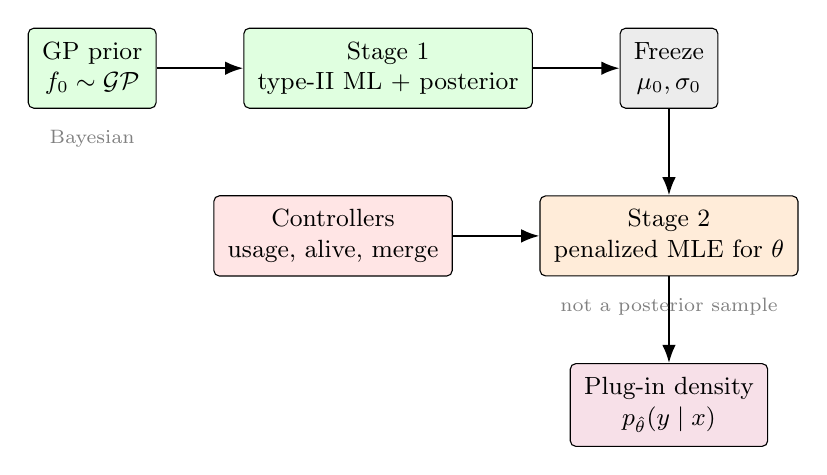
\begin{tikzpicture}[
  box/.style={draw,rounded corners=2pt,align=center,inner sep=5pt,font=\small},
  arr/.style={-{Latex},thick}
]
\node[box,fill=green!12] (prior) {GP prior\\ \(f_0\sim\GP\)};
\node[box,fill=green!12,right=1.1cm of prior] (s1) {Stage 1\\ type-II ML + posterior};
\node[box,fill=gray!15,right=1.1cm of s1] (freeze) {Freeze\\ \(\mu_0,\sigma_0\)};
\node[box,fill=orange!15,below=1.1cm of freeze] (s2) {Stage 2\\ penalized MLE for \(\tht\)};
\node[box,fill=purple!12,below=1.1cm of s2] (pred) {Plug-in density\\ \(p_{\hat\tht}(y\mid x)\)};
\node[box,fill=red!10,left=1.1cm of s2] (ctrl) {Controllers\\ usage, alive, merge};
\draw[arr] (prior) -- (s1);
\draw[arr] (s1) -- (freeze);
\draw[arr] (freeze) -- (s2);
\draw[arr] (s2) -- (pred);
\draw[arr] (ctrl) -- (s2);
\node[below=0.15cm of prior,font=\scriptsize,text=gray] {Bayesian};
\node[below=0.15cm of s2,font=\scriptsize,text=gray] {not a posterior sample};
\end{tikzpicture}
\caption{Only Stage~1 is Bayesian. Stage~2 returns an estimative MoG conditional
(\EBMAP\ if controllers off; controller-modified under champion;
Theorem~\ref{thm:honest}).}
\end{figure}

%==============================================================================
\section*{References}
%==============================================================================
\begin{thebibliography}{99}
\bibitem{Aitchison1975}
J.~Aitchison.
\newblock Goodness of prediction fit.
\newblock \emph{Biometrika}, 62(3):547--554, 1975.
\newblock (Estimative vs.\ Bayesian predictive densities.)

\bibitem{BernardoSmith1994}
J.M.~Bernardo and A.F.M.~Smith.
\newblock \emph{Bayesian Theory}.
\newblock Wiley, 1994.
\newblock (Posterior predictive vs.\ plug-in / estimative prediction.)

\bibitem{Bishop2006}
C.M.~Bishop.
\newblock \emph{Pattern Recognition and Machine Learning}.
\newblock Springer, 2006.
\newblock (Ch.~9: mixture models / mixtures of Gaussians).

\bibitem{GneitingRaftery2007}
T.~Gneiting and A.E.~Raftery.
\newblock Strictly proper scoring rules, prediction, and estimation.
\newblock \emph{Journal of the American Statistical Association}, 102(477):359--378, 2007.

\bibitem{Louizos2018}
C.~Louizos, M.~Welling, and D.P.~Kingma.
\newblock Learning sparse neural networks through \(L_0\) regularization.
\newblock \emph{ICLR}, 2018.

\bibitem{McLachlanPeel2000}
G.~McLachlan and D.~Peel.
\newblock \emph{Finite Mixture Models}.
\newblock Wiley, 2000.

\bibitem{RasmussenGhahramani2001}
C.E.~Rasmussen and Z.~Ghahramani.
\newblock Infinite mixtures of Gaussian process experts.
\newblock In \emph{Advances in Neural Information Processing Systems 14 (NIPS 2001)},
  2002.

\bibitem{RasmussenWilliams2006}
C.E.~Rasmussen and C.K.I.~Williams.
\newblock \emph{Gaussian Processes for Machine Learning}.
\newblock MIT Press, 2006.

\bibitem{Tresp2001}
V.~Tresp.
\newblock Mixtures of Gaussian processes.
\newblock In \emph{Advances in Neural Information Processing Systems 13 (NIPS 2000)},
  pages 654--660, 2001.

\bibitem{YuanNeubauer2009}
C.~Yuan and C.~Neubauer.
\newblock Variational mixture of Gaussian process experts.
\newblock In \emph{Advances in Neural Information Processing Systems 21 (NIPS 2008)},
  pages 1897--1904, 2009.
\end{thebibliography}

\end{document}
